
%% bare_conf.tex
%% V1.3
%% 2007/01/11
%% by Michael Shell
%% See:
%% http://www.michaelshell.org/
%% for current contact information.
%%
%% This is a skeleton file demonstrating the use of IEEEtran.cls
%% (requires IEEEtran.cls version 1.7 or later) with an IEEE conference paper.
%%
%% Support sites:
%% http://www.michaelshell.org/tex/ieeetran/
%% http://www.ctan.org/tex-archive/macros/latex/contrib/IEEEtran/
%% and
%% http://www.ieee.org/

%%*************************************************************************
%% Legal Notice:
%% This code is offered as-is without any warranty either expressed or
%% implied; without even the implied warranty of MERCHANTABILITY or
%% FITNESS FOR A PARTICULAR PURPOSE!
%% User assumes all risk.
%% In no event shall IEEE or any contributor to this code be liable for
%% any damages or losses, including, but not limited to, incidental,
%% consequential, or any other damages, resulting from the use or misuse
%% of any information contained here.
%%
%% All comments are the opinions of their respective authors and are not
%% necessarily endorsed by the IEEE.
%%
%% This work is distributed under the LaTeX Project Public License (LPPL)
%% ( http://www.latex-project.org/ ) version 1.3, and may be freely used,
%% distributed and modified. A copy of the LPPL, version 1.3, is included
%% in the base LaTeX documentation of all distributions of LaTeX released
%% 2003/12/01 or later.
%% Retain all contribution notices and credits.
%% ** Modified files should be clearly indicated as such, including  **
%% ** renaming them and changing author support contact information. **
%%
%% File list of work: IEEEtran.cls, IEEEtran_HOWTO.pdf, bare_adv.tex,
%%                    bare_conf.tex, bare_jrnl.tex, bare_jrnl_compsoc.tex
%%*************************************************************************

% *** Authors should verify (and, if needed, correct) their LaTeX system  ***
% *** with the testflow diagnostic prior to trusting their LaTeX platform ***
% *** with production work. IEEE's font choices can trigger bugs that do  ***
% *** not appear when using other class files.                            ***
% The testflow support page is at:
% http://www.michaelshell.org/tex/testflow/



% Note that the a4paper option is mainly intended so that authors in
% countries using A4 can easily print to A4 and see how their papers will
% look in print - the typesetting of the document will not typically be
% affected with changes in paper size (but the bottom and side margins will).
% Use the testflow package mentioned above to verify correct handling of
% both paper sizes by the user's LaTeX system.
%
% Also note that the "draftcls" or "draftclsnofoot", not "draft", option
% should be used if it is desired that the figures are to be displayed in
% draft mode.
%
\documentclass[conference]{IEEEtran}
% Add the compsoc option for Computer Society conferences.
%
% If IEEEtran.cls has not been installed into the LaTeX system files,
% manually specify the path to it like:
% \documentclass[conference]{../sty/IEEEtran}





% Some very useful LaTeX packages include:
% (uncomment the ones you want to load)


% *** MISC UTILITY PACKAGES ***
%
\usepackage{color}
\usepackage{ifpdf}
\usepackage{filecontents}
% Heiko Oberdiek's ifpdf.sty is very useful if you need conditional
% compilation based on whether the output is pdf or dvi.
% usage:
 \ifpdf
   \usepackage[pdftex]{graphicx}
   \DeclareGraphicsExtensions{.pdf,.PNG,.jpg,.jpeg,.mps, .PNG}
   \usepackage{pgf}
   \usepackage{tikz}
 \else
   \usepackage{graphicx}
   \DeclareGraphicsExtensions{.eps,.bmp}
   \DeclareGraphicsRule{.emf}{bmp}{}{}% declare EMF filename extension
   \DeclareGraphicsRule{.PNG}{bmp}{}{}% declare PNG filename extension
   \usepackage{pgf}
   \usepackage{tikz}
   \usepackage{pstricks}
   % dvi code
 \fi
 \usepackage{epic,bez123}
 \usepackage{floatflt}% package for floatingfigure environment
 \usepackage{wrapfig}% package for wrapfigure environment
% The latest version of ifpdf.sty can be obtained from:
% http://www.ctan.org/tex-archive/macros/latex/contrib/oberdiek/
% Also, note that IEEEtran.cls V1.7 and later provides a builtin
% \ifCLASSINFOpdf conditional that works the same way.
% When switching from latex to pdflatex and vice-versa, the compiler may
% have to be run twice to clear warning/error messages.
\usepackage{verbatimbox}

\usepackage{array}
\newcolumntype{L}[1]{>{\raggedright\let\newline\\\arraybackslash\hspace{0pt}}m{#1}}
\newcolumntype{C}[1]{>{\centering\let\newline\\\arraybackslash\hspace{0pt}}m{#1}}
\newcolumntype{R}[1]{>{\raggedleft\let\newline\\\arraybackslash\hspace{0pt}}m{#1}}


\usepackage[numbers]{natbib}
% *** CITATION PACKAGES ***
%
%\usepackage{cite}
% cite.sty was written by Donald Arseneau
% V1.6 and later of IEEEtran pre-defines the format of the cite.sty package
% \cite{} output to follow that of IEEE. Loading the cite package will
% result in citation numbers being automatically sorted and properly
% "compressed/ranged". e.g., [1], [9], [2], [7], [5], [6] without using
% cite.sty will become [1], [2], [5]--[7], [9] using cite.sty. cite.sty's
% \cite will automatically add leading space, if needed. Use cite.sty's
% noadjust option (cite.sty V3.8 and later) if you want to turn this off.
% cite.sty is already installed on most LaTeX systems. Be sure and use
% version 4.0 (2003-05-27) and later if using hyperref.sty. cite.sty does
% not currently provide for hyperlinked citations.
% The latest version can be obtained at:
% http://www.ctan.org/tex-archive/macros/latex/contrib/cite/
% The documentation is contained in the cite.sty file itself.






% *** GRAPHICS RELATED PACKAGES ***
%
\ifCLASSINFOpdf
  % \usepackage[pdftex]{graphicx}
  % declare the path(s) where your graphic files are
  % \graphicspath{{../pdf/}{../jpeg/}}
  % and their extensions so you won't have to specify these with
  % every instance of \includegraphics
  % \DeclareGraphicsExtensions{.pdf,.jpeg,.png}
\else
  % or other class option (dvipsone, dvipdf, if not using dvips). graphicx
  % will default to the driver specified in the system graphics.cfg if no
  % driver is specified.
  % \usepackage[dvips]{graphicx}
  % declare the path(s) where your graphic files are
  % \graphicspath{{../eps/}}
  % and their extensions so you won't have to specify these with
  % every instance of \includegraphics
  % \DeclareGraphicsExtensions{.eps}
\fi
% graphicx was written by David Carlisle and Sebastian Rahtz. It is
% required if you want graphics, photos, etc. graphicx.sty is already
% installed on most LaTeX systems. The latest version and documentation can
% be obtained at:
% http://www.ctan.org/tex-archive/macros/latex/required/graphics/
% Another good source of documentation is "Using Imported Graphics in
% LaTeX2e" by Keith Reckdahl which can be found as epslatex.ps or
% epslatex.pdf at: http://www.ctan.org/tex-archive/info/
%
% latex, and pdflatex in dvi mode, support graphics in encapsulated
% postscript (.eps) format. pdflatex in pdf mode supports graphics
% in .pdf, .jpeg, .png and .mps (metapost) formats. Users should ensure
% that all non-photo figures use a vector format (.eps, .pdf, .mps) and
% not a bitmapped formats (.jpeg, .png). IEEE frowns on bitmapped formats
% which can result in "jaggedy"/blurry rendering of lines and letters as
% well as large increases in file sizes.
%
% You can find documentation about the pdfTeX application at:
% http://www.tug.org/applications/pdftex





% *** MATH PACKAGES ***
%
\usepackage[cmex10]{amsmath}
% A popular package from the American Mathematical Society that provides
% many useful and powerful commands for dealing with mathematics. If using
% it, be sure to load this package with the cmex10 option to ensure that
% only type 1 fonts will utilized at all point sizes. Without this option,
% it is possible that some math symbols, particularly those within
% footnotes, will be rendered in bitmap form which will result in a
% document that can not be IEEE Xplore compliant!
%
% Also, note that the amsmath package sets \interdisplaylinepenalty to 10000
% thus preventing page breaks from occurring within multiline equations. Use:
%\interdisplaylinepenalty=2500
% after loading amsmath to restore such page breaks as IEEEtran.cls normally
% does. amsmath.sty is already installed on most LaTeX systems. The latest
% version and documentation can be obtained at:
% http://www.ctan.org/tex-archive/macros/latex/required/amslatex/math/





% *** SPECIALIZED LIST PACKAGES ***
%
\usepackage{algorithmic}
% algorithmic.sty was written by Peter Williams and Rogerio Brito.
% This package provides an algorithmic environment fo describing algorithms.
% You can use the algorithmic environment in-text or within a figure
% environment to provide for a floating algorithm. Do NOT use the algorithm
% floating environment provided by algorithm.sty (by the same authors) or
% algorithm2e.sty (by Christophe Fiorio) as IEEE does not use dedicated
% algorithm float types and packages that provide these will not provide
% correct IEEE style captions. The latest version and documentation of
% algorithmic.sty can be obtained at:
% http://www.ctan.org/tex-archive/macros/latex/contrib/algorithms/
% There is also a support site http://matplotlib.org/api/colors_api.htmlat:
% http://algorithms.berlios.de/index.html
% Also of interest may be the (relatively newer and more customizable)
% algorithmicx.sty package by Szasz Janos:
% http://www.ctan.org/tex-archive/macros/latex/contrib/algorithmicx/




% *** ALIGNMENT PACKAGES ***
%
\usepackage{array}
% Frank Mittelbach's and David Carlisle's array.sty patches and improves
% the standard LaTeX2e array and tabular environments to provide better
% appearance and additional user controls. As the default LaTeX2e table
% generation code is lacking to the point of almost being broken with
% respect to the quality of the end results, all users are strongly
% advised to use an enhanced (at the very least that provided by array.sty)
% set of table tools. array.sty is already installed on most systems. The
% latest version and documentation can be obtained at:
% http://www.ctan.org/tex-archive/macros/latex/required/tools/


\usepackage{mdwmath}
%\usepackage{mdwtab}
% Also highly recommended is Mark Wooding's extremely powerful MDW tools,
% especially mdwmath.sty and mdwtab.sty which are used to format equations
% and tables, respectively. The MDWtools set is already installed on most
% LaTeX systems. The lastest version and documentation is available at:
% http://www.ctan.org/tex-archive/macros/latex/contrib/mdwtools/


% IEEEtran contains the IEEEeqnarray family of commands that can be used to
% generate multiline equations as well as matrices, tables, etc., of high
% quality.


\usepackage{eqparbox}
% Also of notable interest is Scott Pakin's eqparbox package for creating
% (automatically sized) equal width boxes - aka "natural width parboxes".
% Available at:
% http://www.ctan.org/tex-archive/macros/latex/contrib/eqparbox/





% *** SUBFIGURE PACKAGES ***
\usepackage[tight,footnotesize]{subfigure}
% subfigure.sty was written by Steven Douglas Cochran. This package makes it
% easy to put subfigures in your figures. e.g., "Figure 1a and 1b". For IEEE
% work, it is a good idea to load it with the tight package option to reduce
% the amount of white space around the subfigures. subfigure.sty is already
% installed on most LaTeX systems. The latest version and documentation can
% be obtained at:
% http://www.ctan.org/tex-archive/obsolete/macros/latex/contrib/subfigure/
% subfigure.sty has been superceeded by subfig.sty.



%\usepackage[caption=false]{caption}
%\usepackage[font=footnotesize]{subfig}
% subfig.sty, also written by Steven Douglas Cochran, is the modern
% replacement for subfigure.sty. However, subfig.sty requires and
% automatically loads Axel Sommerfeldt's caption.sty which will override
% IEEEtran.cls handling of captions and this will result in nonIEEE style
% figure/table captions. To prevent this problem, be sure and preload
% caption.sty with its "caption=false" package option. This is will preserve
% IEEEtran.cls handing of captions. Version 1.3 (2005/06/28) and later
% (recommended due to many improvements over 1.2) of subfig.sty supports
% the caption=false option directly:
%\usepackage[caption=false,font=footnotesize]{subfig}
%
% The latest version and documentation can be obtained at:
% http://www.ctan.org/tex-archive/macros/latex/contrib/subfig/
% The latest version and documentation of caption.sty can be obtained at:
% http://www.ctan.org/tex-archive/macros/latex/contrib/caption/


\usepackage{caption}
\usepackage{tikz}
\def\checkmark{\tikz\fill[scale=0.4](0,.35) -- (.25,0) -- (1,.7) -- (.25,.15) -- cycle;}

% *** FLOAT PACKAGES ***
%
%\usepackage{fixltx2e}
% fixltx2e, the successor to the earlier fix2col.sty, was written by
% Frank Mittelbach and David Carlisle. This package corrects a few problems
% in the LaTeX2e kernel, the most notable of which is that in current
% LaTeX2e releases, the ordering of single and double column floats is not
% guaranteed to be preserved. Thus, an unpatched LaTeX2e can allow a
% single column figure to be placed prior to an earlier double column
% figure. The latest version and documentation can be found at:
% http://www.ctan.org/tex-archive/macros/latex/base/



%\usepackage{stfloats}
% stfloats.sty was written by Sigitas Tolusis. This package gives LaTeX2e
% the ability to do double column floats at the bottom of the page as well
% as the top. (e.g., "\begin{figure*}[!b]" is not normally possible in
% LaTeX2e). It also provides a command:
%\fnbelowfloat
% to enable the placement of footnotes below bottom floats (the standard
% LaTeX2e kernel puts them above bottom floats). This is an invasive package
% which rewrites many portions of the LaTeX2e float routines. It may not work
% with other packages that modify the LaTeX2e float routines. The latest
% version and documentation can be obtained at:
% http://www.ctan.org/tex-archive/macros/latex/contrib/sttools/
% Documentation is contained in the stfloats.sty comments as well as in the
% presfull.pdf file. Do not use the stfloats baselinefloat ability as IEEE
% does not allow \baselineskip to stretch. Authors submitting work to the
% IEEE should note that IEEE rarely uses double column equations and
% that authors should try to avoid such use. Do not be tempted to use the
% cuted.sty or midfloat.sty packages (also by Sigitas Tolusis) as IEEE does
% not format its papers in such ways.





% *** PDF, URL AND HYPERLINK PACKAGES ***
%
%\usepackage{url}
% url.sty was written by Donald Arseneau. It provides better support for
% handling and breaking URLs. url.sty is already installed on most LaTeX
% systems. The latest version can be obtained at:
% http://www.ctan.org/tex-archive/macros/latex/contrib/misc/
% Read the url.sty source comments for usage information. Basically,
% \url{my_url_here}.





% *** Do not adjust lengths that control margins, column widths, etc. ***
% *** Do not use packages that alter fonts (such as pslatex).         ***
% There should be no need to do such things with IEEEtran.cls V1.6 and later.
% (Unless specifically asked to do so by the journal or conference you plan
% to submit to, of course. )


% correct bad hyphenation here
\hyphenation{op-tical net-works semi-conduc-tor}

\begin{document}
%
% paper title
% can use linebreaks \\ within to get better formatting as desired
\title{Incorporating Multiple Cluster Models for Network Traffic Classification}


% author names and affiliations
% use a multiple column layout for up to three different
% affiliations
\author{\IEEEauthorblockN{Anil Kumar, Jinoh Kim, Sang C. Suh}
	\IEEEauthorblockA
	{Department of Computer Science \\
		Texas A\&M University,
		Commerce, TX\\
		Email:akatta1@leomail.tamuc.edu, \\
		jinoh.kim@tamuc.edu, sang.suh@tamuc.edu}
	\and
	\IEEEauthorblockN{Ganho Choi}
	\IEEEauthorblockA{Sysmate Inc.\\
		1290 Dunsan-Dong Seo-Gu, Deajeon, 302-830, Korea\\
		Email: ghchoi@sysmate.com}
}
% conference papers do not typically use \thanks and this command
% is locked out in conference mode. If really needed, such as for
% the acknowledgment of grants, issue a \IEEEoverridecommandlockouts
% after \documentclass

% for over three affiliations, or if they all won't fit within the width
% of the page, use this alternative format:
%
%\author{\IEEEauthorblockN{Michael Shell\IEEEauthorrefmark{1},
%Homer Simpson\IEEEauthorrefmark{2},
%James Kirk\IEEEauthorrefmark{3},
%Montgomery Scott\IEEEauthorrefmark{3} and
%Eldon Tyrell\IEEEauthorrefmark{4}}
%\IEEEauthorblockA{\IEEEauthorrefmark{1}School of Electrical and Computer Engineering\\
%Georgia Institute of Technology,
%Atlanta, Georgia 30332--0250\\ Email: see http://www.michaelshell.org/contact.html}
%\IEEEauthorblockA{\IEEEauthorrefmark{2}Twentieth Century Fox, Springfield, USA\\
%Email: homer@thesimpsons.com}
%\IEEEauthorblockA{\IEEEauthorrefmark{3}Starfleet Academy, San Francisco, California 96678-2391\\
%Telephone: (800) 555--1212, Fax: (888) 555--1212}
%\IEEEauthorblockA{\IEEEauthorrefmark{4}Tyrell Inc., 123 Replicant Street, Los Angeles, California 90210--4321}}




% use for special paper notices
%\IEEEspecialpapernotice{(Invited Paper)}




% make the title area
\maketitle

\begin{abstract}
	%Identifying applications are critical for a broad range of network related activities like bandwidth usage, security etc. Earlier, applications are identified based on port numbers, which proved to be not accurate anymore; based of payload signatures, which is proved to be accurate but has been limited in the real world implementation because of privacy concerns; based on flow statistics, which uses machine learning algorithms to find the patterns in the flow statistics and use it in classification, which has been widely used for many classification problems.  In this research, we explore the importance of the attributes or a combination of flow attributes which can classify applications effectively. The idea is to combine clustering and using combinations of flow attributes and we measure accuracy of each combination. We are currently evaluating our model with real-world traffic traces indicating effectiveness of the selective attributes is effective than using the whole set of attributes.
%	Network traffic classification is one of essential functions for local and ISP networks for quality of service, network usage statistics, resource provisioning, and security. 
%With its importance, a substantial number of previous studies have explored various machine learning techniques based on network flow statistics to improve the accuracy of classification and reported promising results with fairly high classification accuracy. However, what we observed from previously proposed network traffic classification techniques with our own data set recently collected are somewhat unacceptable results. In particular, we observed that simply combining flow attributes for classification may lead to unexpectedly poor accuracy in classification (less than xx\%).
%	In this paper, we propose a new traffic classification method based on attribute groups, each of which consists of a set of attributes belonging to a single parameter (e.g., packet size, inter-arrival time, etc).
%	Our method then incorporates multiple cluster models obtained from individual attribute groups to reach the final classification decision based on the population of candidate protocols (or applications).
%	From our extensive experiments, we observed that our proposed technique significantly outperforms existing cluster-based classification techniques, showing up to yy\% better accuracy.

Network traffic classification is one of essential functions for local and ISP networks for quality of service, network usage statistics, resource provisioning, and security.
With its importance, a substantial number of previous studies have explored various machine learning techniques based on network flow statistics to improve the accuracy of classification, and using a semi-supervised learning with clustering is one branch of research directions.
However, we observed fairly unacceptable results (around 85\% on average and 91\% at best) with previously proposed techniques based on clustering.
In particular, simply combining flow attributes for clustering leads to unexpectedly poor accuracy in classification (less than 70\%).

With these observations, we first examine the impact of attributes to the classification performance, and then
propose a new technique based on multiple trained cluster models to take multiple sets of combinations of attributes into account for classification, rather than simply merging the attributes in a single model.
Our proposed technique also includes a selection step to reach to the final classification decision from the multiple models, and we explore a set of selection strategies.
From our extensive experiments, we observed that our proposed technique significantly outperforms existing cluster-based techniques, showing up to 95\% classification accuracy.

\end{abstract}
% IEEEtran.cls defaults to using nonbold math in the Abstract.
% This preserves the distinction between vectors and scalars. However,
% if the conference you are submitting to favors bold math in the abstract,
% then you can use LaTeX's standard command \boldmath at the very start
% of the abstract to achieve this. Many IEEE journals/conferences frown on
% math in the abstract anyway.

% no keywords




% For peer review papers, you can put extra information on the cover
% page as needed:
% \ifCLASSOPTIONpeerreview
% \begin{center} \bfseries EDICS Category: 3-BBND \end{center}
% \fi
%
% For peerreview papers, this IEEEtran command inserts a page break and
% creates the second title. It will be ignored for other modes.
% \IEEEpeerreviewmaketitle



\section{Introduction}

Accurately identifying network-based applications is of major interest for local and ISP networks for various purposes, including
quality of service, network usage statistics, resource provisioning, and security~\cite{Bernaille:2006:EAI:1368436.1368445, DBLP:conf/iwcmc/GrimaudoMB12, DBLP:conf/infocom/XieIKFN12}.
Earlier, network protocols/applications were identified simply based on TCP/UDP port numbers.
%, but the traditional identification technique is no longer reliable since many of existing and newly emerging network applications allow dynamic port selection without relying on standard port numbers~\cite{Ohzahata:2005, BitTorrentProto}.
However, the traditional technique based on port-numbers are proved to be ineffective where accuracy is less than 70\%~\cite{ACAS} since network applications using random port numbers or non-standard port numbers are increasing day-by-day and also usage of tunneling makes identification of applications more difficult just based on port numbers.
Due to this reason, a substantial body of research has been conducted to replace or complement the port-based identification.

One approach to overcome the limitation of the port-based identification is to inspect the packet payload information with template signature sets~\cite{conf/IEEEcit/YeXWP09,DBLP:conf/noms/ParkWKH08} or machine learning techniques~\cite{ACAS}.
While highly accurate,  drawbacks of the deep packet inspection-based approach include encrypted traffic transformed with cryptographic keys and privacy concerns as many countries do not permit the extraction of full payload information from packets with increasing privacy requirements.

The limitations of the traditional port-based identification and the payload inspection-based classification suggested to utilize  transport layer characteristics of the application as the differentiator. From previously proposed techniques~\cite{}, we can see the combination of transport layer characteristics with machine learning techniques would be an effective alternative for network traffic classification. %accurately identifies the applications, with accuracies comparable to that of payload-based signature matching.
Several techniques were proposed based on supervised learning~\cite{}, while some other techniques utilized unsupervised or semi-supervised clustering techniques~\cite{}, reporting promising  accuracy for network traffic classification.
However, what we actually observed from previously proposed network traffic classification techniques with our own data set recently collected are somewhat unacceptable results. In particular, one important observation is that simply combining flow attributes for classification leads to unexpectedly poor accuracy in classification (less than xx\%), which motivates us to thoroughly examine the impact of flow attributes in this work.\footnote{A (network) flow is defined as a set of packets for a single session of communication with the five tuples of source IP address, destination IP address, source port number, destination port number, and protocol type.}

%An alternative approach is to utilize machine learning-based classification techniques with flow statistics, such as flow size, flow duration, packet size, packet inter-arrival time, and so forth, without having privacy concerns~\cite{}.

To evaluate the significance of flow attributes to classification accuracy, we use a notion of attribute groups.
%In this paper, we propose a new traffic classification method based on clustering with the
An attribute group consists of a set of attributes that are derived from a single communication characteristic.
For example, the packet size group includes the minimum packet size, maximum packet size, average packet size, standard deviation of packet sizes observed from a single flow.
We consider four attribute groups of flow information group, packet size group, packet inter-arrival time group, and relative packet inter-arrival time group, as will be discussed in the Section~\ref{sec:grouping} in detail.
From our preliminary experiments, we observed that some combinations of attributes work quite better than the other combinations.
Moreover, simply applying a subset of attributes selected based on the evaluation to supervised techniques significantly improves performance compared to using the entire attributes without selection.
With the initial observations, we developed a new semi-supervised learning technique based on the attribute groups.
A key challenge for this approach is how to use multiple attribute groups to make a single classification decision.
To address this, we establish independent cluster models based on individual attribute groups and incorporate the results collected from multiple cluster models.
Although it is known that clustering techniques generally work poorly compared to supervised learning techniques~\cite{DBLP:conf/infocom/XieIKFN12}, we will present that the proposed technique using multiple cluster models yield comparable classification accuracy.

The key contributions of this paper can be summarized as follows:

\begin{itemize}
	\item We evaluate the significance of flow attributes to classification accuracy with a notion of attribute group.
	We used 18 flow attributes in total and four groups are formed, which are flow information group, packet size group, packet inter-arrival time group, and relative packet inter-arrival time group.
	\item From the evaluation results with the attribute groups, we examine classification accuracy with the entire attributes and with the selected ones using supervised learning methods, to ensure  validity of the selection.
	\item We present a new clustering technique for network traffic classification that utilizes multiple cluster models developed from the attribute groups. A set of heuristic algorithms are also presented to incorporate multiple cluster models.
	\item We also present experimental results for evaluating the proposed traffic classification technique. Experiments for sensitivity study are also conducted to see the impact of configurable parameters. Note that we repeated the same experiments at least five times and report the average to consider variations.
\end{itemize}

The paper organization is as follows. We provide a summary of related studies
in Section~\ref{sec:related}.
In Section~\ref{sec:grouping}, we examine the significance of attribute groups to classification accuracy and performance with selected attributes with supervised learning methods.
We then present the new clustering technique incorporating multiple cluster models in Section~\ref{sec:multi_cluster} and evaluation results are presented in Section~\ref{sec:eval}.
Finally we conclude our presentation with a summary and future direction in Section~\ref{sec:conc}.

\section{Related Work}
\label{sec:related}
%\subsection{Related Study}
%Existing techniques based on port-numbers are proved to be very ineffective where accuracy is less than 70 \cite{}, as number of applications using random port numbers or non-standard port numbers are increasing day-by-day and also usage of tunneling makes identification of application more difficult just based on port numbers.
%
%To counter drawbacks of port-based application identification, many payload-based techniques have been proposed\cite{}. In payload-based technique, payload of the flow will be extracted and searched for known signature of the applications. Results indicate that this method is very effective with high accuracies. Drawbacks include encrypted traffic, and wide deployment of tools based on payload signature is a problem as many countries doesn't allow the extraction of full payload from packets due to privacy concerns
%
%Drawbacks of both payload-based signature matching and port-based classification led us to use the transport layer characteristics of the application as the differentiator of the application. From various proposed techniques\cite{} we can see combination of transport layer characteristics in combination with Machine learning techniques accurately identifies the applications, with accuracies comparable to that of payload-based signature matching.

A substantial body of research has been conducted for network traffic classification with machine learning techniques.
The work can broadly be divided into the following three categories:

\begin{itemize} \itemsep3pt \parskip3pt \parsep3pt
	\item \emph{Un-supervised}~\cite{}:
	Labeling information of the training data is not available at the time of training. We use various clustering algorithms for the classification of unlabeled data\cite{}.
	\item \emph{Supervised}~\cite{}:
	We provide the labels for the flows when we train the model and then use this model to test each incoming flow whether it belongs to any of the application which is provided at the time of training\cite{}.
	\item \emph{Semi-supervised}~\cite{}:
	We provide partial labeling information at the time of training and we use clustering algorithms to cluster the training data. We use the partially available labeling information to label each cluster. Heuristics have been proposed on how to label the cluster from partial training information\cite{}
\end{itemize}

%We extensively ran existing techniques\cite{} against our dataset. We ran supervised (Adaboost, Naive Bayes), unsupervised (K-Means using all attributes of the flow statistics) and Early Application Identification (K-Means using only Average Packet Size as the attribute for the machine learning algorithm).

\textbf{ACAS}\cite{ACAS}: ACAS encodes initial \textit{n-bytes} of the payload into space and uses supervised machine learning algorithm as the classification algorithm. We observe this technique is effective in identifying applications with very high accuracy with our data set ($\approx$ 99\%). Drawback of this technique is it requires completely labeled data. Which means we should know prior to the start classification it should know all the applications that classifier may encounter in future (which is not a feasible solution). It also
As mentioned, however, it requires the access to the payload, which could be limited by laws due to privacy concerns. In addition, encryption plays an important role in classification, which may significantly lower the accuracy.

\textbf{K-Means classification technique}\cite{Erman:2006:TCU:1162678.1162679}.
%We ran K-Means classification technique, where we use all the available 18 attributes of flow statistics for the classification. We ran experiments to study the effect of the number of clusters\cite{}.
We ran the K-Means classification technique across by varying the number of clusters from 10 to 140, and Figure~\ref{fig:k_means_all} show the result.
As can be seen from the figure, classification performance is largely not acceptable with quite less than 70\% accuracy.
%In fig.\ref{fig:k_means_all} K-Means all Attrs is the accuracy of the existing technique \cite{} and K-Means Selected is the accuracy when we consider only subset of total attributes, based on the selection strategy which we suggested later in the paper. We observe the accuracy of the existing technique is low in comparison with the accuracy of the clustering technique when we consider only subset of the attributes.


\textbf{Early Application Identification}.\cite{Bernaille:2006:EAI:1368436.1368445}
%We ran Early Application Identification\cite{} against our dataset. Instead of considering \emph{Average Packet Size} for first 4 packets as suggested in the paper\cite{}, we considered whole packets \emph{Average Packet Size} of the flow. It can observed from fig.\ref{fig:early_app_identification} that the accuracy increases slowly with increase in the percent of the training set.
We also evaluated this technique. Rather than considering only the first 4 packets in a flow as suggested in the paper, we considered the whole packets to see the maximum performance.
Although this technique is based on clustering as the above technique and uses only the average packet size attribute, it yielded quite enhanced results as shown in Figure~\ref{fig:early_app_identification} across diverse ratios between training data set and testing data set.

%\begin{figure}[!t]
%	\centering
%	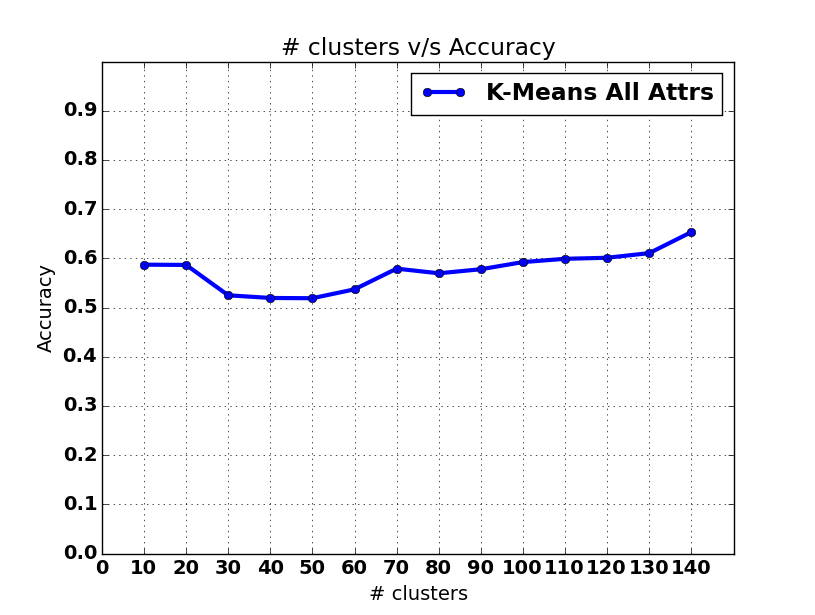
\includegraphics[width=1\columnwidth]{k_means_selected_all}
%	% where an .eps filename suffix will be assumed under latex,
%	% and a .pdf suffix will be assumed for pdflatex; or what has been declared
%	% via \DeclareGraphicsExtensions.
%	\caption{Number of clusters v/s Accuracy for K-Means algorithm with All}
%	\label{fig:k_means_all}
%\end{figure}
%
%\begin{figure}[!t]
%	\centering
%	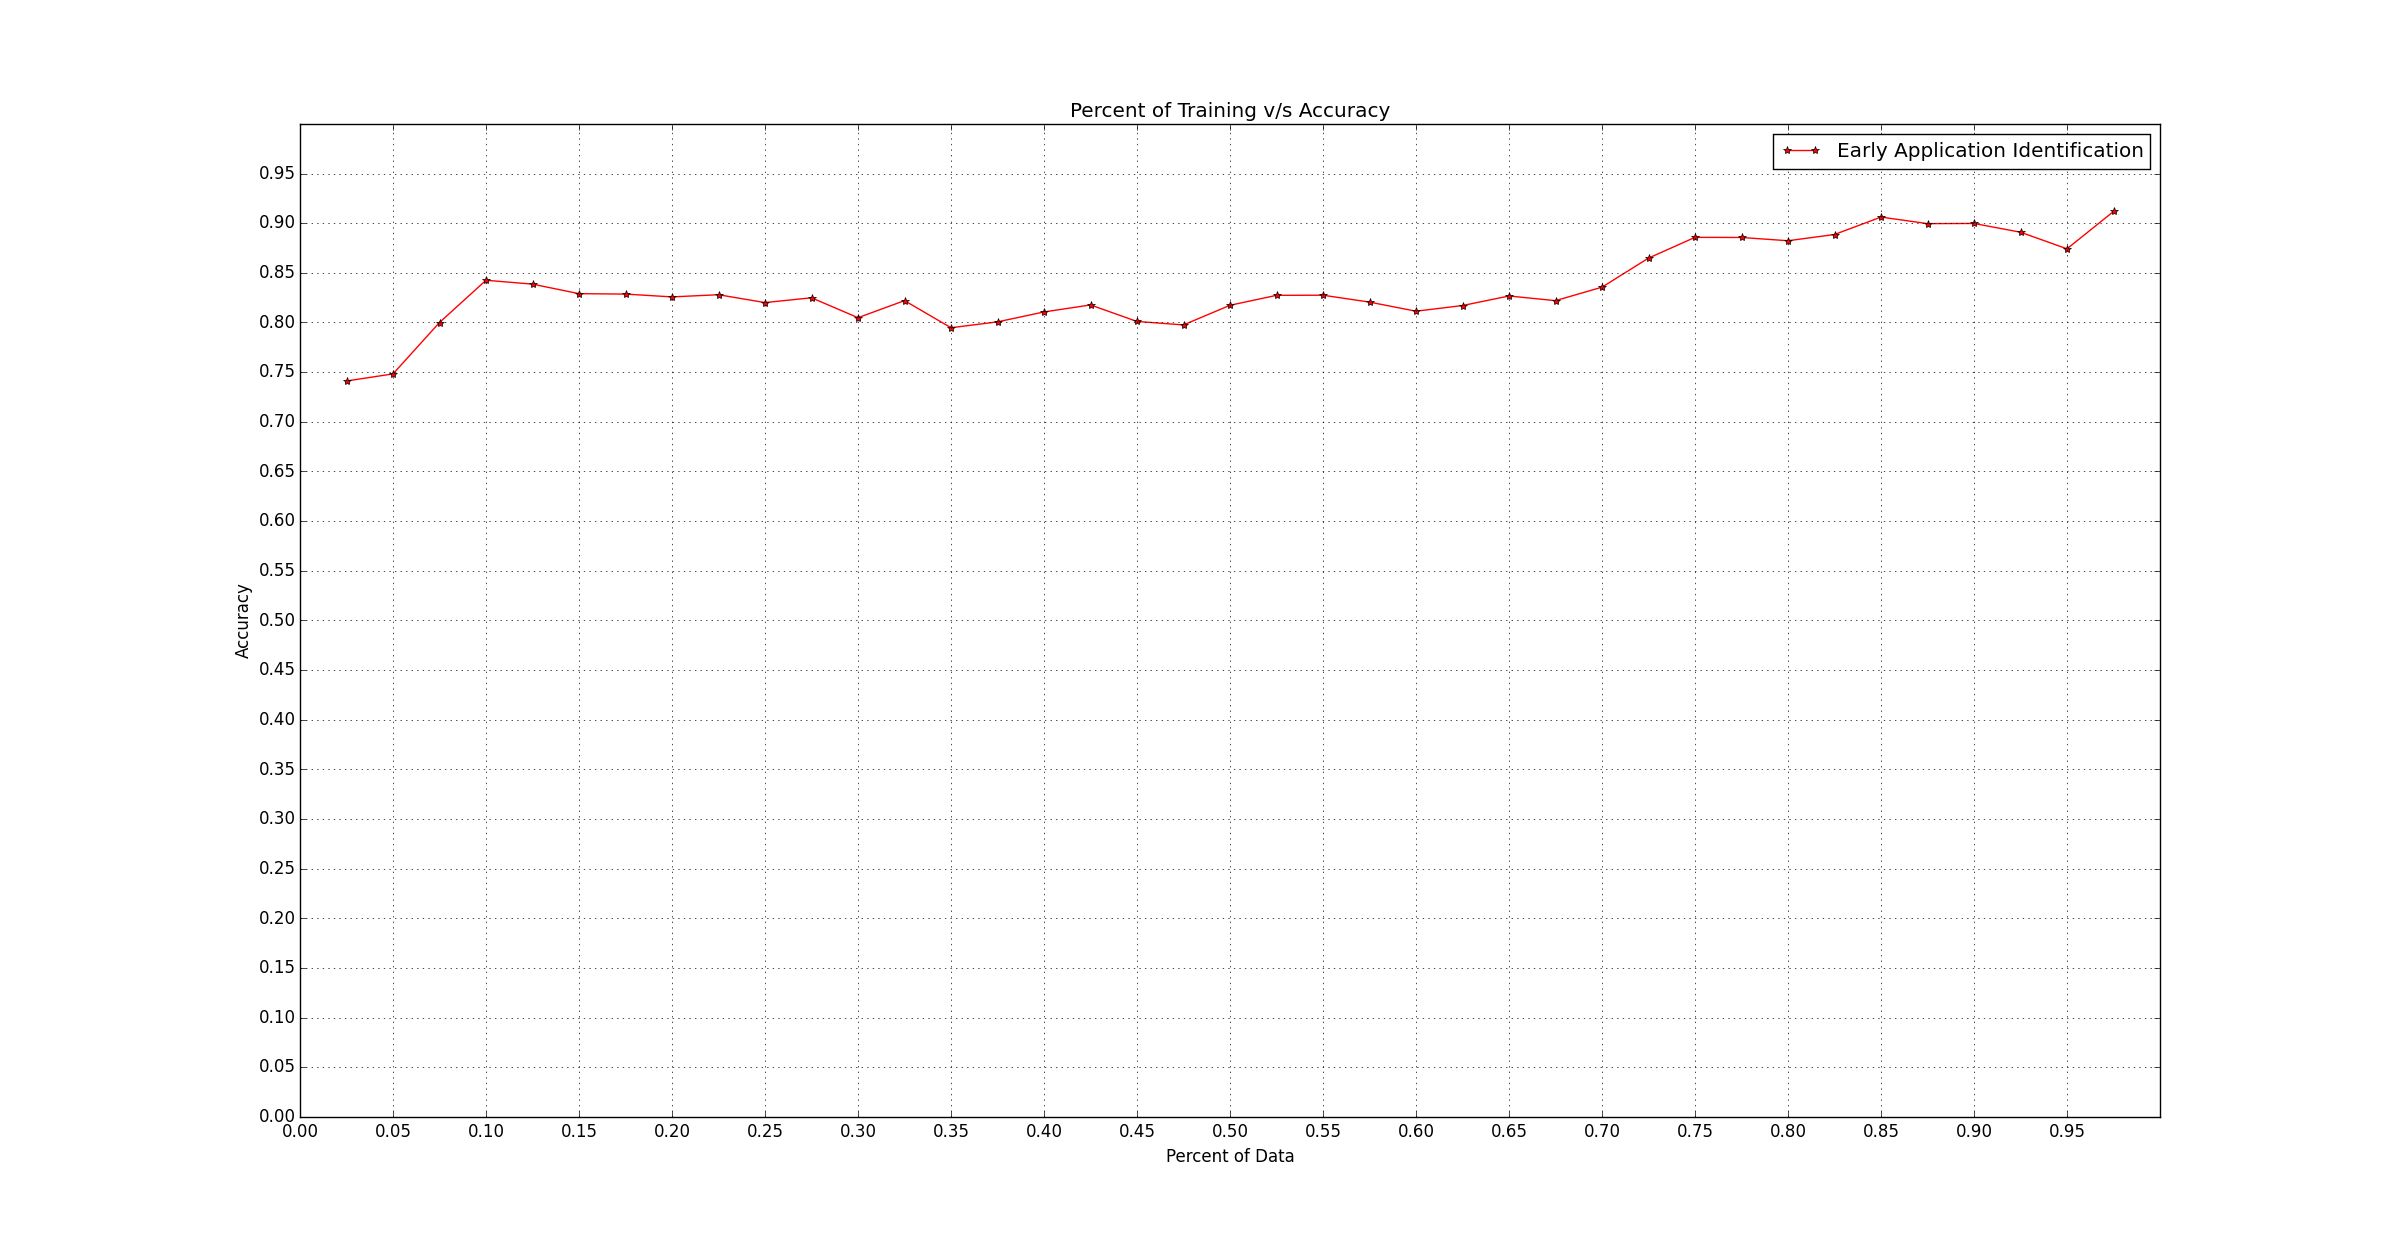
\includegraphics[width=1\columnwidth]{early_application_result}
%	% where an .eps filename suffix will be assumed under latex,
%	% and a .pdf suffix will be assumed for pdflatex; or what has been declared
%	% via \DeclareGraphicsExtensions.
%	\caption{Percentage of Training Data v/s Accuracy for Early Application Identification}
%	\label{fig:early_app_identification}
%\end{figure}


\begin{figure*}[t]
 \centering
 \subfigure[K-mean clustering~\cite{Erman:2006:TCU:1162678.1162679}] {
    \label{fig:k_means_all}
    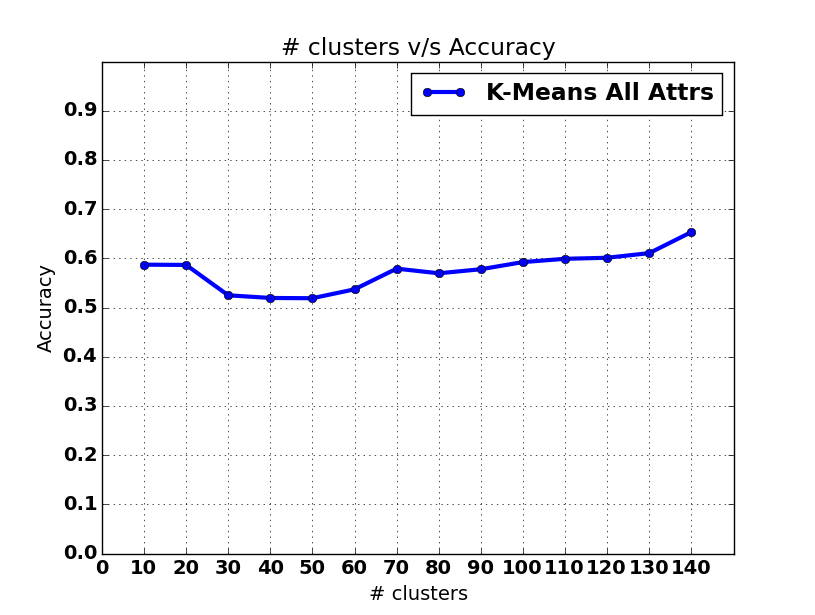
\includegraphics[width=0.45\textwidth]{k_means_selected_all}}
 \hspace{.3in}
 \subfigure[Early identification~\cite{Bernaille:2006:EAI:1368436.1368445}] {
    \label{fig:early_app_identification}
    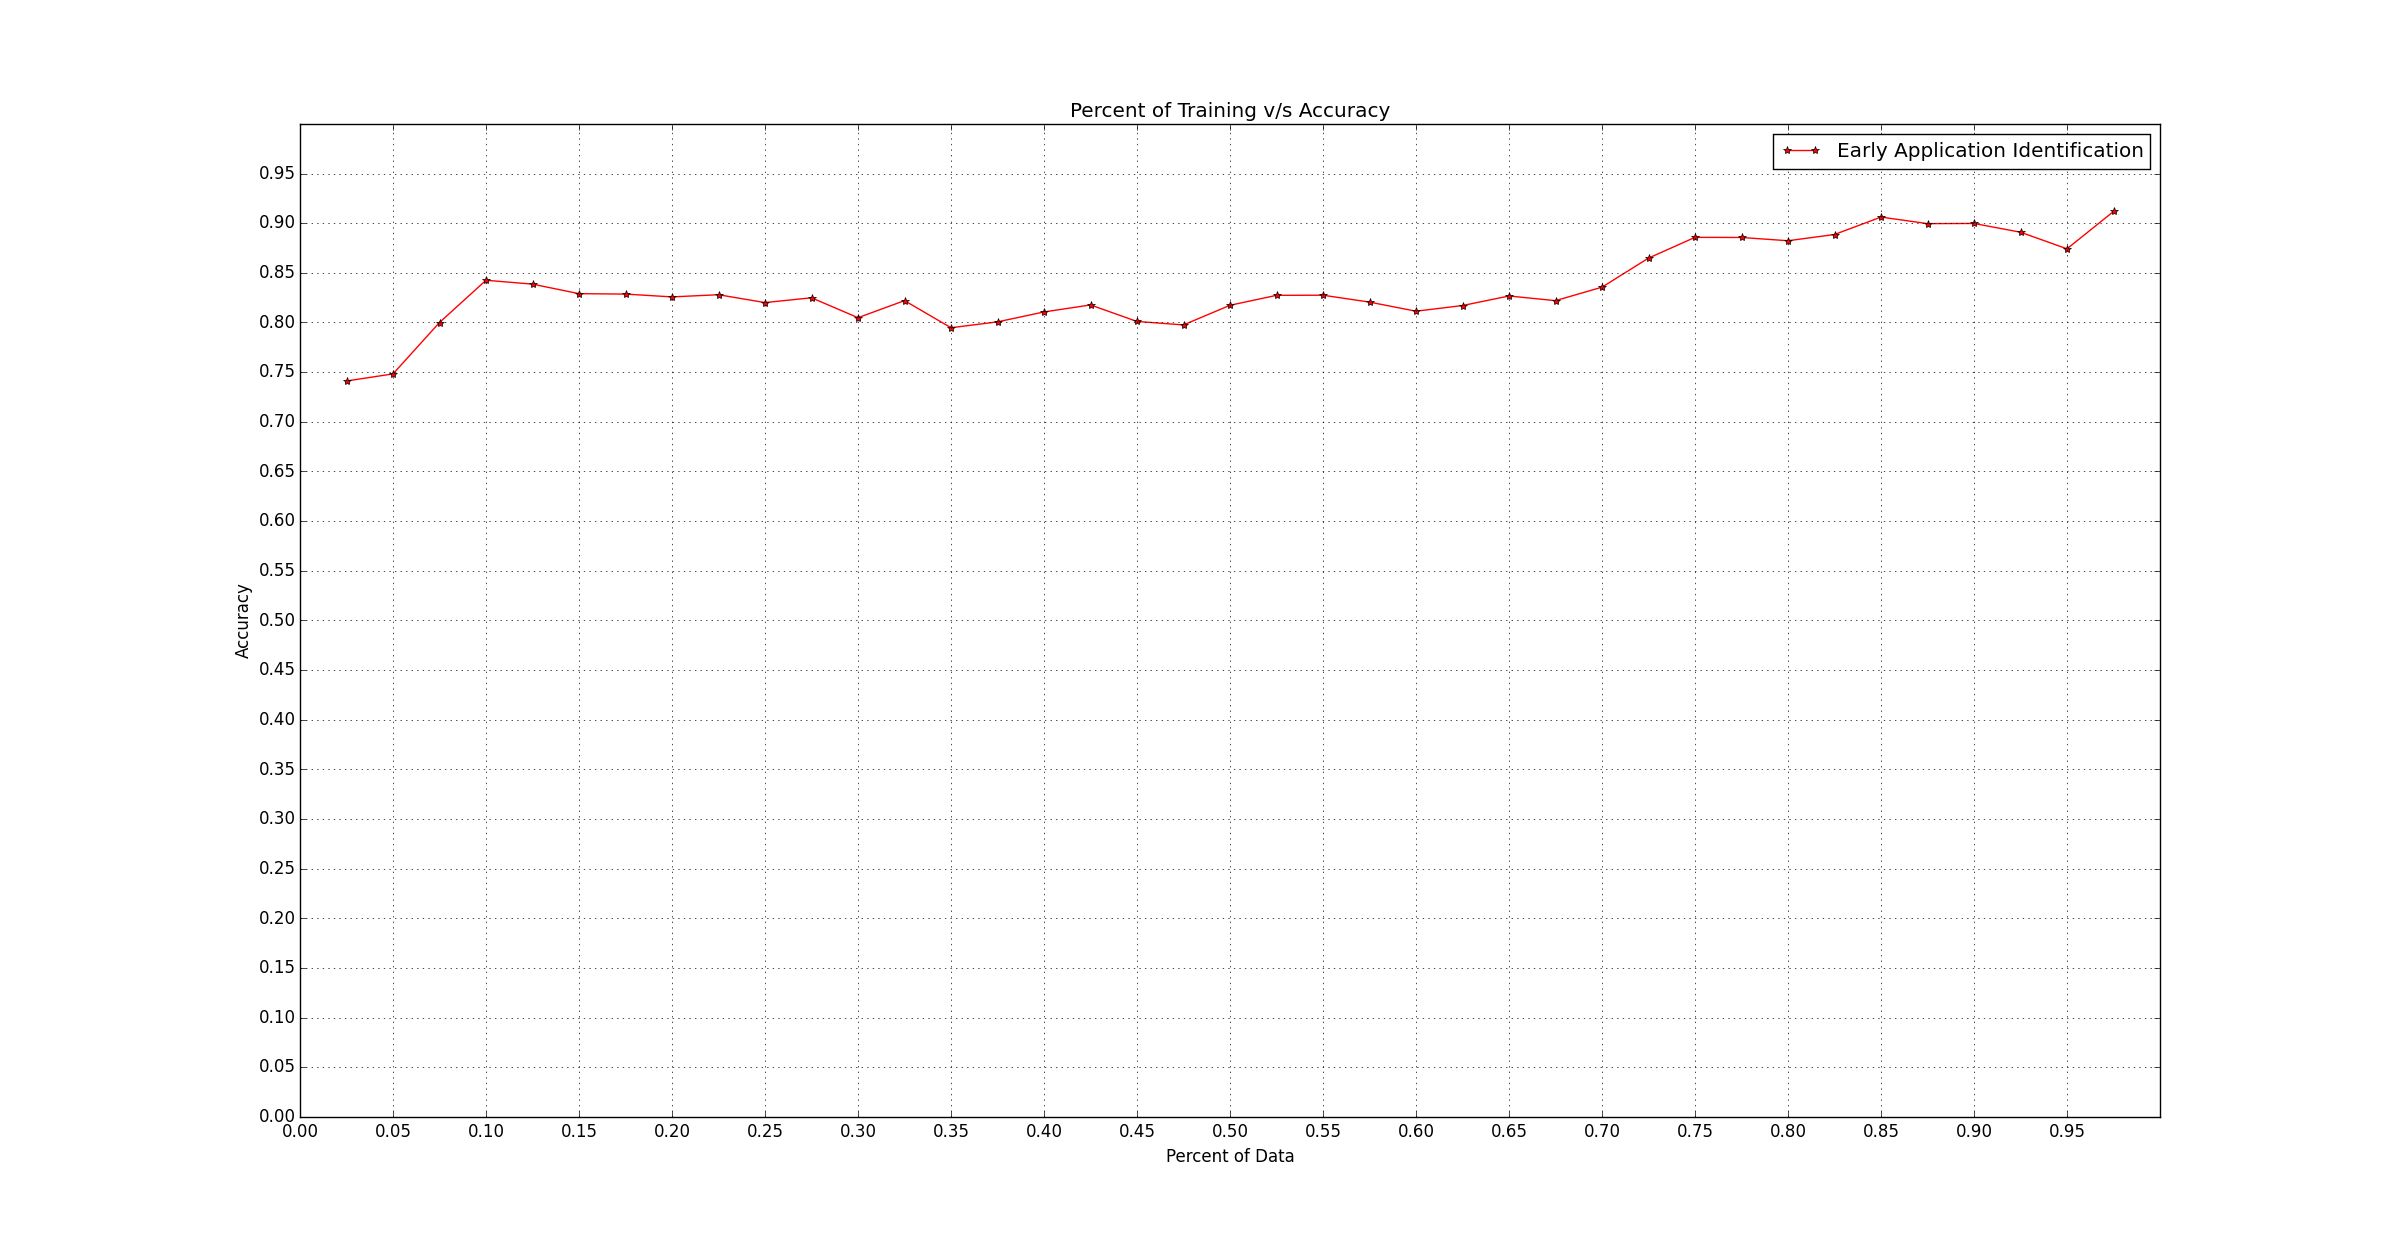
\includegraphics[width=0.45\textwidth]{early_application_result}}
 \caption{Network traffic classification with previous techniques
 }
 \label{fig:previous}
\end{figure*}



\section{Grouping of Attributes}
\label{sec:grouping}

In this section, we present the impact of flow statistics attributes to classification accuracy based on grouping of attributes.
We first describe the flow attributes used in this study and attribute groups, and then discuss classification accuracy for individual groups.

From the network traffic data set, totally 18 flow attributes are considered, as summarized in Table~\ref{tab:attrs}.
The information about the data set used in this study will be described in Section~\ref{sec:eval} in detail.

\renewcommand{\arraystretch}{1.5}
%\begin{table*}
%	\caption{Attributes used in out studies}
%	\label{table_attributes_description}
%	\begin{tabular}{|c|L{2.8in}|L{2.8in}|}
%		\hline Name & Description & Related Attributes \\
%		\hline IAT  & Inter Arrival Time, time difference between $i^{th}$ and $i+1^{th}$ packets & Standard Deviation IAT\newline Minimum IAT\newline Maximum IAT\newline Average IAT \\
%		\hline RIAT & Relative Inter Arrival Time, IAT of the the packet divided my mimimum of IAT & Average RIAT\newline Standard Deviation of RIAT\newline Minimum RIAT\newline Maximum of RIAT \\
%		\hline Packet Size & Size of the packet in the flow including headers & Average Packet Size\newline Standard Deviation of Packet Size\newline Minimum Packet Size\newline Maximum Packet Size \\
%		\hline Flow Duration & Duration of the entire flow from initiation to termination & Flow Duration\\
%		\hline Total Packet Size & Summation of the packet sizes of all the packets inside the flow & Total Packet Size \\
%		\hline Number of Packets & Total number of packets inside the flow & Number of Packets \\
%		\hline Packets per Second & $ \frac{Number of Packets}{Flow Duration} $ & Average Packets Per Second\\
%		\hline Bytes Per Second & $ \frac{Total Packet Size}{Flow Duration} $ & Average Bytes Per Second \\
%		\hline Payload Size & $Size_{Paload Size} = Size_{Total} - Size_{header } $ & Payload Size \\
%		\hline
%	\end{tabular}
%	%\begin{tabular}{|c|c|}
%	%	\hline  Average IAT & Maximum of IAT \\ [2pt]
%	%	\hline  Minimum of IAT & Stadard Deviation of IAT\\
%	%	\hline  Average RIAT & Maximum of RIAT\\
%	%	\hline  Minimum of RIAT& Standard Deviation of RIAT\\
%	%	\hline  Average Packet Size & Minimum of Packet Size \\
%	%	\hline  Maximum of Packet Size & Standard Deviation of Packet Size \\
%	%	\hline  Total Packet Size& Flow Duration\\
%	%	\hline  Number of Packets & Average Packets/second\\
%	%	\hline  Average Bytes/second & Payload Size \\
%	%	\hline
%%	\end{tabular}
%\end{table*}
\begin{table*}
    \centering
	\caption{Attributes used in out studies}
	\begin{tabular}{|l|l|p{12cm}|}
%	\begin{tabular}{|p{2cm}|p{6cm}|}
		\hline Attribute & Type & Description  \\ \hline
		\hline Flow size & flow level & Total number of bytes in the flow \\
		\hline Flow duration & flow level & Duration of the  flow from initiation to termination \\
%		\hline Total packet size & Summation of the packet sizes of all the packets inside the flow \\
		\hline Number of Packets & flow level & Total number of packets inside the flow  \\
		\hline Number of packets per second & flow level & Number of packets / Flow duration \\
		\hline Number of bytes Per second & flow level & Total packet size / Flow duration \\
		\hline Payload size & flow level & the payload size in bytes without network and transport layer headers \\
		\hline Packet size & packet level & min/max packet size and average and standard deviation of packet sizes in the flow  \\
		\hline Packet inter-arrival time (IAT) & packet level & min/max packet inter-arrival time and average and standard deviation of inter-arrival times in the flow  \\
		\hline Relative IAT (RIAT) & packet level & Recomputation of IAT after dividing IAT by round-trip delay:  max RIAT and average and standard deviation of RIATs \\
		\hline
	\end{tabular}
	\label{tab:attrs}
\end{table*}


%\vspace{5pt}
%\begin{itemize} \itemsep3pt \parskip3pt \parsep3pt
%	\item \emph{Flow Size}
%	Total number of bytes transferred during the entire flow.
%	\item \emph{Flow Duration}
%	Difference between time when last packet of the flow captured and first packet of flow captured
%	\item \emph{Packet Size and it's variations}
%	Size of the each packet. We can get \emph{minimum}, \emph{maximum}, \emph{Average} and \emph{Standard deviation} by using all the packets of the flow.
%	\item \emph{Inter Arrival Time and it's variations}
%	Inter Arrival Time($\tau'$)\cite{} is the time difference between $\tau_{next}$ - $\tau_{current}$.
%	\item \emph{Relative Inter Arrival Time and it's variations} \cite{}
%	Relative inter arrival time is defined as
%	$$\tau'_i = \frac{\tau_i}{\displaystyle \min_{k=1..|f|-1}{\tau_k}}$$
%	Here, $f$ is a flow with $|f|$ number of packets and $\tau_i$ is the time difference between $i$-th packet and $(i+1)$-th packet in that flow.\cite{}
%\end{itemize}

As discussed in the previous section, using only a single attribute of average packet size works much better than using a greater number of attributes for traffic classification.
Thus, it would be good to see the significance of the attributes.
Since there can exist too many combinations of the attributes, we categorized the attributes into four groups based on their characteristics, as follows:

\begin{itemize} \itemsep3pt \parskip3pt \parsep3pt
	\item \emph{Flow group}: Any flow-level attribute belongs to this group, including flow size, flow duration, and so forth.
	\item \emph{Packet size group}: Attributes related to packet size belong to this group: \emph{minimum}, \emph{maximum}, \emph{average}, and \emph{standard deviation} packet size
	\item \emph{Inter-Arrival Time (IAT) group}: Attributes from inter-arrival time: \emph{minimum}, \emph{maximum}, \emph{average}, and \emph{standard deviation} inter-arrival time
\item \emph{Relative Inter-Arrival Time (RIAT) group}: Attributes related to relative inter-arrival time: \emph{maximum}, \emph{average}, and \emph{standard deviation}. Relative inter-arrival time is defined as,
	$$\tau'_i = \frac{\tau_i}{\displaystyle \min_{k=1..|f|-1}{\tau_k}}$$
	Here, $f$ is a flow with $|f|$ number of packets and $\tau_i$ is the time difference between $i$-th packet and $(i+1)$-th packet in that flow.
\end{itemize}

%\subsection{Preliminary Results}
%Our experiments results for each group of attributes are as following:

To evaluate the attributes' performance impact to network classification, we applied the clustering technique introduced in the previous section with the individual subsets of attributes for each group.
To measure classification accuracy, we used a simple metric of true positive, and thus, accuracy indicates true positive rate in this paper.
We used our own data set described in the evaluation section in detail (Section~\ref{sec:eval}).
By default, we used 90\%:10\% for the ratio of the number of training flows to the number of test flows.
Thus, the results with the default training set ratio would be the approximations of the maximum classification accuracy since using a smaller set of training flows generally leads to worse accuracy in classification.


%\renewcommand{\arraystretch}{1.0}
\begin{table}
    \centering
	\caption{Accuracy of flow group}
	\label{table_flow_group}
%	\tabcolsep=0.40cm
%	\begin{tabular}{|c|c|C{0.8in}|c|c|c|c|}
	\begin{tabular}{|C{0.35in}|C{0.35in}|C{0.35in}|C{0.35in}|C{0.35in}|C{0.35in}|C{0.35in}|}
		\hline Flow Size & Flow Duration & Number of Packets &  Avg Pkts Per Sec & Avg Bytes Per Sec & Payload Size & Accuracy \\
		%\hline\checkmark & $\times$ & $\times$ & $\times$ & $\times$ & $\times$ & 89.05\% \\
		%\hline$\times$ & \checkmark & $\times$ & $\times$ & $\times$ & $\times$ & 40.72\% \\
		%\hline$\times$ & $\times$ & \checkmark & $\times$ & $\times$ & $\times$ & 59.54\% \\
		%\hline$\times$ & $\times$ & $\times$ & \checkmark & $\times$ & $\times$ & 44.98\% \\
		%\hline$\times$ & $\times$ & $\times$ & $\times$ & \checkmark & $\times$ & 50.48\% \\
	%	\hline$\times$ & $\times$ & $\times$ & $\times$ & $\times$ & \checkmark & 89.43\% \\
		\hline\checkmark & \checkmark & $\times$ & $\times$ & $\times$ & $\times$ & 92.92\% \\
		\hline\checkmark & $\times$ & \checkmark & $\times$ & $\times$ & $\times$ & 91.66\% \\
		\hline\checkmark & $\times$ & $\times$ & \checkmark & $\times$ & $\times$ & 91.12\% \\
		%\hline\checkmark & $\times$ & $\times$ & $\times$ & \checkmark & $\times$ & 49.91\% \\
		\hline\checkmark & $\times$ & $\times$ & $\times$ & $\times$ & \checkmark & 94.53\% \\
		%\hline$\times$ & \checkmark & \checkmark & $\times$ & $\times$ & $\times$ & 60.99\% \\
		%\hline$\times$ & \checkmark & $\times$ & \checkmark & $\times$ & $\times$ & 45.13\% \\
		%\hline$\times$ & \checkmark & $\times$ & $\times$ & \checkmark & $\times$ & 49.29\% \\
		\hline$\times$ & \checkmark & $\times$ & $\times$ & $\times$ & \checkmark & 92.58\% \\
		%\hline$\times$ & $\times$ & \checkmark & \checkmark & $\times$ & $\times$ & 50.00\% \\
		%\hline$\times$ & $\times$ & \checkmark & $\times$ & \checkmark & $\times$ & 50.68\% \\
		\hline$\times$ & $\times$ & \checkmark & $\times$ & $\times$ & \checkmark & 93.80\% \\
		%\hline$\times$ & $\times$ & $\times$ & \checkmark & \checkmark & $\times$ & 49.74\% \\
	%	\hline$\times$ & $\times$ & $\times$ & \checkmark & $\times$ & \checkmark & 87.07\% \\
		%\hline$\times$ & $\times$ & $\times$ & $\times$ & \checkmark & \checkmark & 50.94\% \\
	%	\hline\checkmark & \checkmark & \checkmark & $\times$ & $\times$ & $\times$ & 89.95\% \\
		\hline\checkmark & \checkmark & $\times$ & \checkmark & $\times$ & $\times$ & 92.31\% \\
		%\hline\checkmark & \checkmark & $\times$ & $\times$ & \checkmark & $\times$ & 49.88\% \\
	%	\hline\checkmark & \checkmark & $\times$ & $\times$ & $\times$ & \checkmark & 89.54\% \\
	%	\hline\checkmark & $\times$ & \checkmark & \checkmark & $\times$ & $\times$ & 86.20\% \\
		%\hline\checkmark & $\times$ & \checkmark & $\times$ & \checkmark & $\times$ & 49.81\% \\
	%	\hline\checkmark & $\times$ & \checkmark & $\times$ & $\times$ & \checkmark & 87.25\% \\
		%\hline\checkmark & $\times$ & $\times$ & \checkmark & \checkmark & $\times$ & 50.58\% \\
	%	\hline\checkmark & $\times$ & $\times$ & \checkmark & $\times$ & \checkmark & 88.83\% \\
		%\hline\checkmark & $\times$ & $\times$ & $\times$ & \checkmark & \checkmark & 49.14\% \\
		%\hline$\times$ & \checkmark & \checkmark & \checkmark & $\times$ & $\times$ & 47.74\% \\
		%\hline$\times$ & \checkmark & \checkmark & $\times$ & \checkmark & $\times$ & 49.67\% \\
		\hline$\times$ & \checkmark & \checkmark & $\times$ & $\times$ & \checkmark & 92.02\% \\
		%\hline$\times$ & \checkmark & $\times$ & \checkmark & \checkmark & $\times$ & 49.40\% \\
	%	\hline$\times$ & \checkmark & $\times$ & \checkmark & $\times$ & \checkmark & 89.36\% \\
		%\hline$\times$ & \checkmark & $\times$ & \checkmark & $\times$ & \checkmark & 50.17\% \\
		%\hline$\times$ & $\times$ & \checkmark & \checkmark & \checkmark & $\times$ & 49.45\% \\
	%	\hline$\times$ & $\times$ & \checkmark & \checkmark & $\times$ & \checkmark & 88.46\% \\
		%\hline$\times$ & $\times$ & \checkmark & $\times$ & \checkmark & \checkmark & 51.83\% \\
		%\hline$\times$ & $\times$ & $\times$ & \checkmark & \checkmark & \checkmark & 50.90\% \\
		\hline\checkmark & \checkmark & \checkmark & \checkmark & $\times$ & $\times$ & 91.86\% \\
		%\hline\checkmark & \checkmark & \checkmark & $\times$ & \checkmark & $\times$ & 49.30\% \\
	%	\hline\checkmark & \checkmark & \checkmark & $\times$ & $\times$ & \checkmark & 81.47\% \\
		%\hline\checkmark & \checkmark & $\times$ & \checkmark & \checkmark & $\times$ & 49.64\% \\
	%	\hline\checkmark & \checkmark & $\times$ & \checkmark & $\times$ & \checkmark & 85.54\% \\
	%	\hline\checkmark & \checkmark & $\times$ & $\times$ & \checkmark & \checkmark & 51.12\% \\
	%	\hline\checkmark & $\times$ & \checkmark & \checkmark & \checkmark & $\times$ & 49.76\% \\
	%	\hline\checkmark & $\times$ & \checkmark & \checkmark & $\times$ & \checkmark & 83.67\% \\
	%	\hline\checkmark & $\times$ & \checkmark & $\times$ & \checkmark & \checkmark & 50.40\% \\
	%	\hline\checkmark & $\times$ & $\times$ & \checkmark & \checkmark & \checkmark & 50.46\% \\
	%	\hline$\times$ & \checkmark & \checkmark & \checkmark & \checkmark & $\times$ & 50.33\% \\
	%	\hline$\times$ & \checkmark & \checkmark & \checkmark & $\times$ & \checkmark & 87.11\% \\
	%	\hline$\times$ & \checkmark & \checkmark & $\times$ & \checkmark & \checkmark & 51.16\% \\
	%	\hline$\times$ & \checkmark & $\times$ & \checkmark & \checkmark & \checkmark & 51.54\% \\
	%	\hline$\times$ & $\times$ & \checkmark & \checkmark & \checkmark & \checkmark & 51.18\% \\
	%	\hline\checkmark & \checkmark & \checkmark & \checkmark & \checkmark & $\times$ & 49.20\% \\
	%	\hline\checkmark & \checkmark & \checkmark & \checkmark & $\times$ & \checkmark & 80.33\% \\
	%	\hline\checkmark & \checkmark & \checkmark & $\times$ & \checkmark & \checkmark & 49.41\% \\
	%	\hline\checkmark & \checkmark & $\times$ & \checkmark & \checkmark & \checkmark & 50.08\% \\
	%	\hline\checkmark & $\times$ & \checkmark & \checkmark & \checkmark & \checkmark & 51.12\% \\
	%	\hline$\times$ & \checkmark & \checkmark & \checkmark & \checkmark & \checkmark & 51.92\% \\
	%	\hline\checkmark & \checkmark & \checkmark & \checkmark & \checkmark & \checkmark & 50.93\% \\
		\hline
	\end{tabular}
\end{table}

%\renewcommand{\arraystretch}{1.5}
\begin{table}
    \centering
	\caption{Accuracy of packet size group}
	\label{table_pkt_size_group}
	\tabcolsep=0.01cm
	\begin{tabular}{|c|c|c|c|c|}
		\hline Avg Pkt Size & Min Pkt Size & Max Pkt Size & Stddev Pkt Size & Final Accuracy \\
		\hline \checkmark & $\times$ & $\times$ & $\times$ & 92.43\% \\
		\hline $\times$ & \checkmark & $\times$ & $\times$ & 75.95\% \\
		\hline $\times$ & $\times$ & \checkmark & $\times$ & 92.22\% \\
		\hline $\times$ & $\times$ & $\times$ & \checkmark & 91.82\% \\
		\hline \checkmark & \checkmark & $\times$ & $\times$ & 91.46\% \\
		\hline \checkmark & $\times$ & \checkmark & $\times$ & 92.98\% \\
		\hline \checkmark & $\times$ & $\times$ & \checkmark & 93.96\% \\
		\hline $\times$ & \checkmark & \checkmark & $\times$ & 91.46\% \\
		\hline $\times$ & \checkmark & $\times$ & \checkmark & 92.69\% \\
		\hline $\times$ & $\times$ & \checkmark & \checkmark & 92.76\% \\
		\hline \checkmark & \checkmark & \checkmark & $\times$ & 93.98\% \\
		\hline \checkmark & \checkmark & $\times$ & \checkmark & 93.62\% \\
		\hline \checkmark & $\times$ & \checkmark & \checkmark & 92.76\% \\
		\hline $\times$ & \checkmark & \checkmark & \checkmark & 91.73\% \\
		\hline \checkmark & \checkmark & \checkmark & \checkmark & 93.75\% \\
		\hline
	\end{tabular}
\end{table}


%\renewcommand{\arraystretch}{1.5}
\begin{table}
    \centering
	\caption{Accuracy of IAT group}
	\label{table_iat_group}
	\begin{tabular}{|c|c|c|c|c|}
		\hline Avg IAT & Min IAT & Max IAT & Stddev IAT & Final Accuracy \\
		\hline \checkmark & $\times$ & $\times$ & $\times$ & 47.29\% \\
		\hline $\times$ & \checkmark & $\times$ & $\times$ & 49.34\% \\
		\hline $\times$ & $\times$ & \checkmark & $\times$ & 39.20\% \\
		\hline $\times$ & $\times$ & $\times$ & \checkmark & 42.82\% \\
		\hline \checkmark & \checkmark & $\times$ & $\times$ & 45.86\% \\
		\hline \checkmark & $\times$ & \checkmark & $\times$ & 44.25\% \\
		\hline \checkmark & $\times$ & $\times$ & \checkmark & 47.78\% \\
		\hline $\times$ & \checkmark & \checkmark & $\times$ & 39.64\% \\
		\hline $\times$ & \checkmark & $\times$ & \checkmark & 42.91\% \\
		\hline $\times$ & $\times$ & \checkmark & \checkmark & 40.54\% \\
		\hline \checkmark & \checkmark & \checkmark & $\times$ & 45.20\% \\
		\hline \checkmark & \checkmark & $\times$ & \checkmark & 47.18\% \\
		\hline \checkmark & $\times$ & \checkmark & \checkmark & 42.70\% \\
		\hline $\times$ & \checkmark & \checkmark & \checkmark & 40.10\% \\
		\hline \checkmark & \checkmark & \checkmark & \checkmark & 42.75\% \\
		\hline
	\end{tabular}
\end{table}

%\renewcommand{\arraystretch}{1.5}
\begin{table}
    \centering
	\caption{Accuracy of RIAT group}
	\label{table_riat_group}
	\begin{tabular}{|c|c|c|c|c|}
		\hline Avg RIAT & Max RIAT& Stddev RIAT & Final Accuracy \\
		\hline \checkmark & $\times$ & $\times$ & 55.86\% \\
		\hline $\times$ & \checkmark & $\times$ & 54.08\% \\
		\hline $\times$ & $\times$ & \checkmark & 53.41\% \\
		\hline \checkmark & \checkmark & $\times$ & 55.21\% \\
		\hline \checkmark & $\times$ & \checkmark & 54.28\% \\
		\hline $\times$ & \checkmark & \checkmark & 55.25\% \\
		\hline \checkmark & \checkmark & \checkmark & 56.41\% \\
		\hline
	\end{tabular}
\end{table}

Table~\ref{table_flow_group} shows accuracy of classification when using a subset of attributes in the flow group.
In fact, there can exist many number of combinations with the six attributes in the flow group, but we report the top 10 results only to save the space.
Surprisingly, we can see very high accuracy up to 94.5\% with only 2--4 attributes in the flow group.

We next examined the attributes in the packet size group.
As shown in Table~\ref{table_pkt_size_group}, any combination of attributes in the packet size group works very good, showing up to 94\% accuracy.
When using minimum packet size only, it does not work well with 76\% accuracy.
The results here explain why it worked well only with the attribute of average packet size in \cite{Bernaille:2006:EAI:1368436.1368445}.
We observed the combination of \emph{Avg Pkt Size} and \emph{Stddev Pkt Size} gives the best accuracy of the group, and the combination of \emph{Min Pkt Size}, \emph{Max Pkt Size} and \emph{Avg Pkt Size} gives the second best accuracy in this group.

Unlike the flow group and the packet size group, we observed that the attributes related to packet inter-arrival time are not good with clearly low classification accuracy less than 60\%, even with 90\% training flows (out of the total flows).
Hence, the groups are less attractive for network traffic classification than the flow and packet groups.

%As shown in Table~\ref{table_iat_group} and Table~\ref{table_riat_group}, classification accuracy remained below 60\% with any combination of the attributes in each group of
%We observe from Table~\ref{table_iat_group}, Table~\ref{table_riat_group}, Table~\ref{table_flow_group} and Table~\ref{table_pkt_size_group} that accuracy is not very good when we consider all the attributes of flow in the classification. When subset of attributes in a group is considered then the accuracy is better than when all attributes in the group are considered. From Table~\ref{table_iat_group}, Table~\ref{table_riat_group} accuracy is very low, this group doesn't make much difference in the accuracy when considered in the classification. From Table~\ref{table_flow_group} and Table~\ref{table_pkt_size_group} we observe accuracy when considering all the attributes is not as good as when we consider subset of them. Table~\ref{table_pkt_size_group} we observe combination of \emph{Avg Pkt Size} and \emph{Stddev Pkt Size} gives the best accuracy of the group, similarly combination of \emph{Min Pkt Size}, \emph{Max Pkt Size} and \emph{Avg Pkt Size} gives second best accuracy of the group. Similarly from Table~\ref{table_flow_group} combination of \emph{Total Pkt Size}, \emph{Payload Size} and also combination of \emph{Payload size}, \emph{Number of Packets in the flow} gives better accuracy in the group.



%\begin{figure}[!t]
%	\centering
%	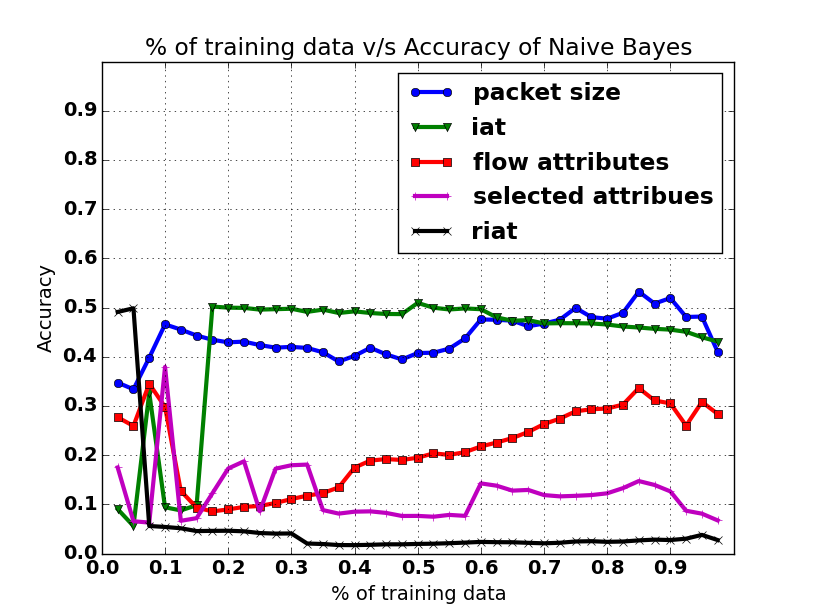
\includegraphics[width=1\columnwidth]{naive_bayes_all_attr_plot.png}
%	% where an .eps filename suffix will be assumed under latex,
%	% and a .pdf suffix will be assumed for pdflatex; or what has been declared
%	% via \DeclareGraphicsExtensions.
%	\caption{\% of training data v/s Accuracy for Naive Bayes with Groups of Attributes. Plotting Naive Bayes with each group of attributes.}
%	\label{fig:naive_attributes}
%\end{figure}
%\begin{figure}[!t]
%	\centering
%	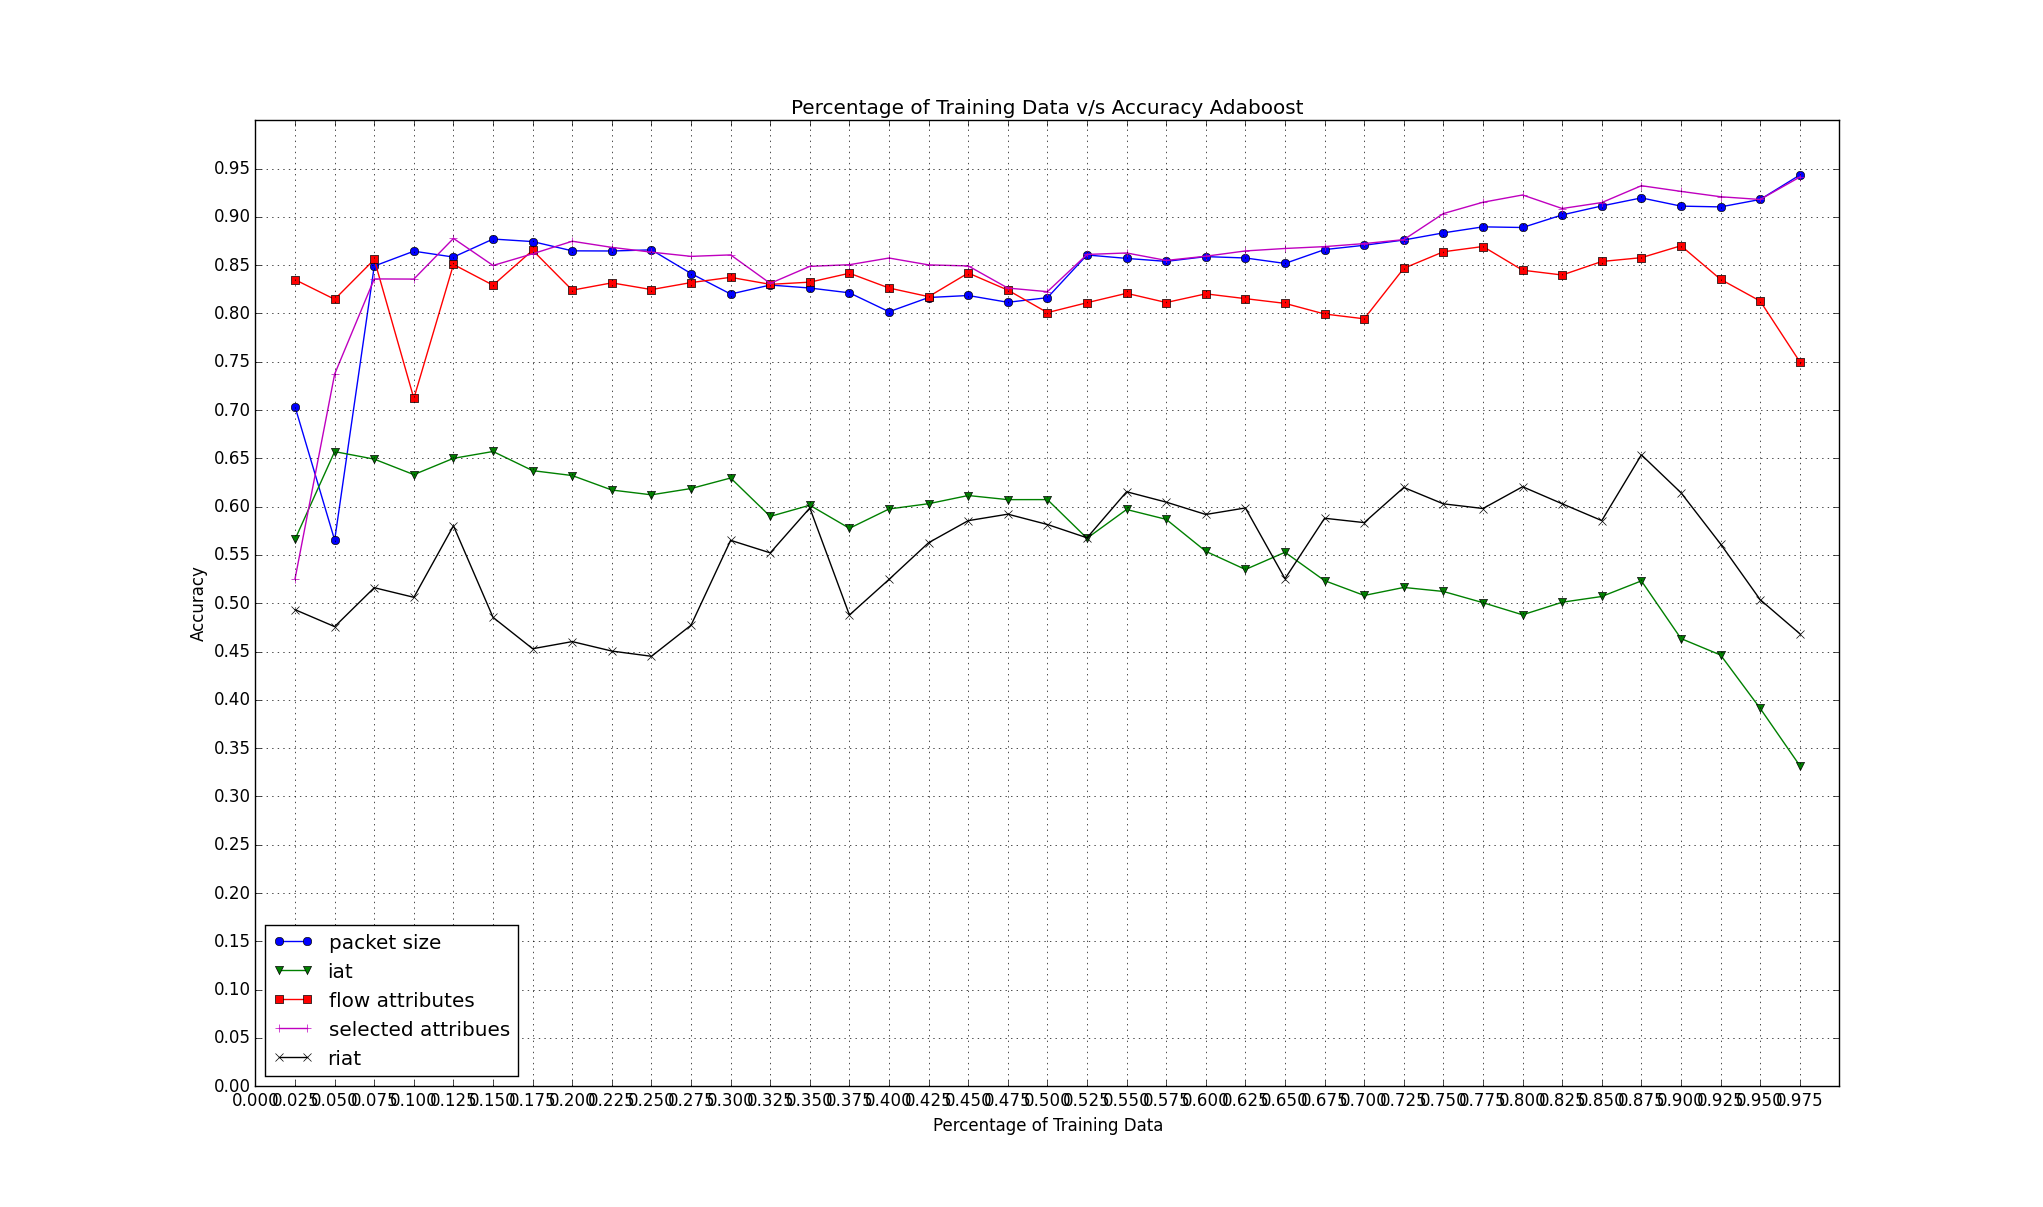
\includegraphics[width=1\columnwidth]{adaboost_all_attr_plot.png}
%	% where an .eps filename suffix will be assumed under latex,
%	% and a .pdf suffix will be assumed for pdflatex; or what has been declared
%	% via \DeclareGraphicsExtensions.
%	\caption{Percent of training data v/s Accuracy for Adaboost with Groups of Attributes.Plotting Adaboost with each group of attributes.}
%	\label{fig:adaboost_attributes}
%\end{figure}

\begin{figure*}[t]
 \centering
 \subfigure[Naive Bayes classifier] {
    \label{fig:naive_attributes}
    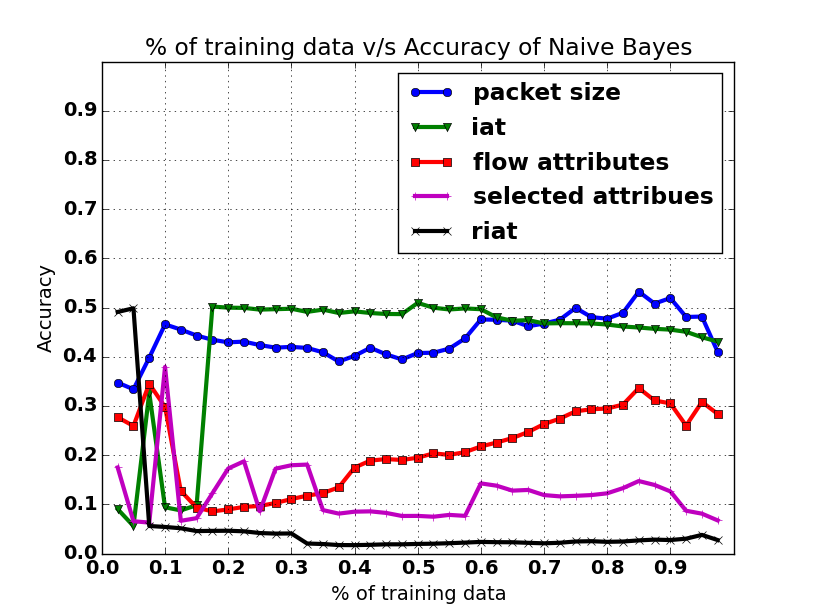
\includegraphics[width=0.45\textwidth]{naive_bayes_all_attr_plot.png}}
 \hspace{.3in}
 \subfigure[Adaboost classifier] {
    \label{fig:adaboost_attributes}
    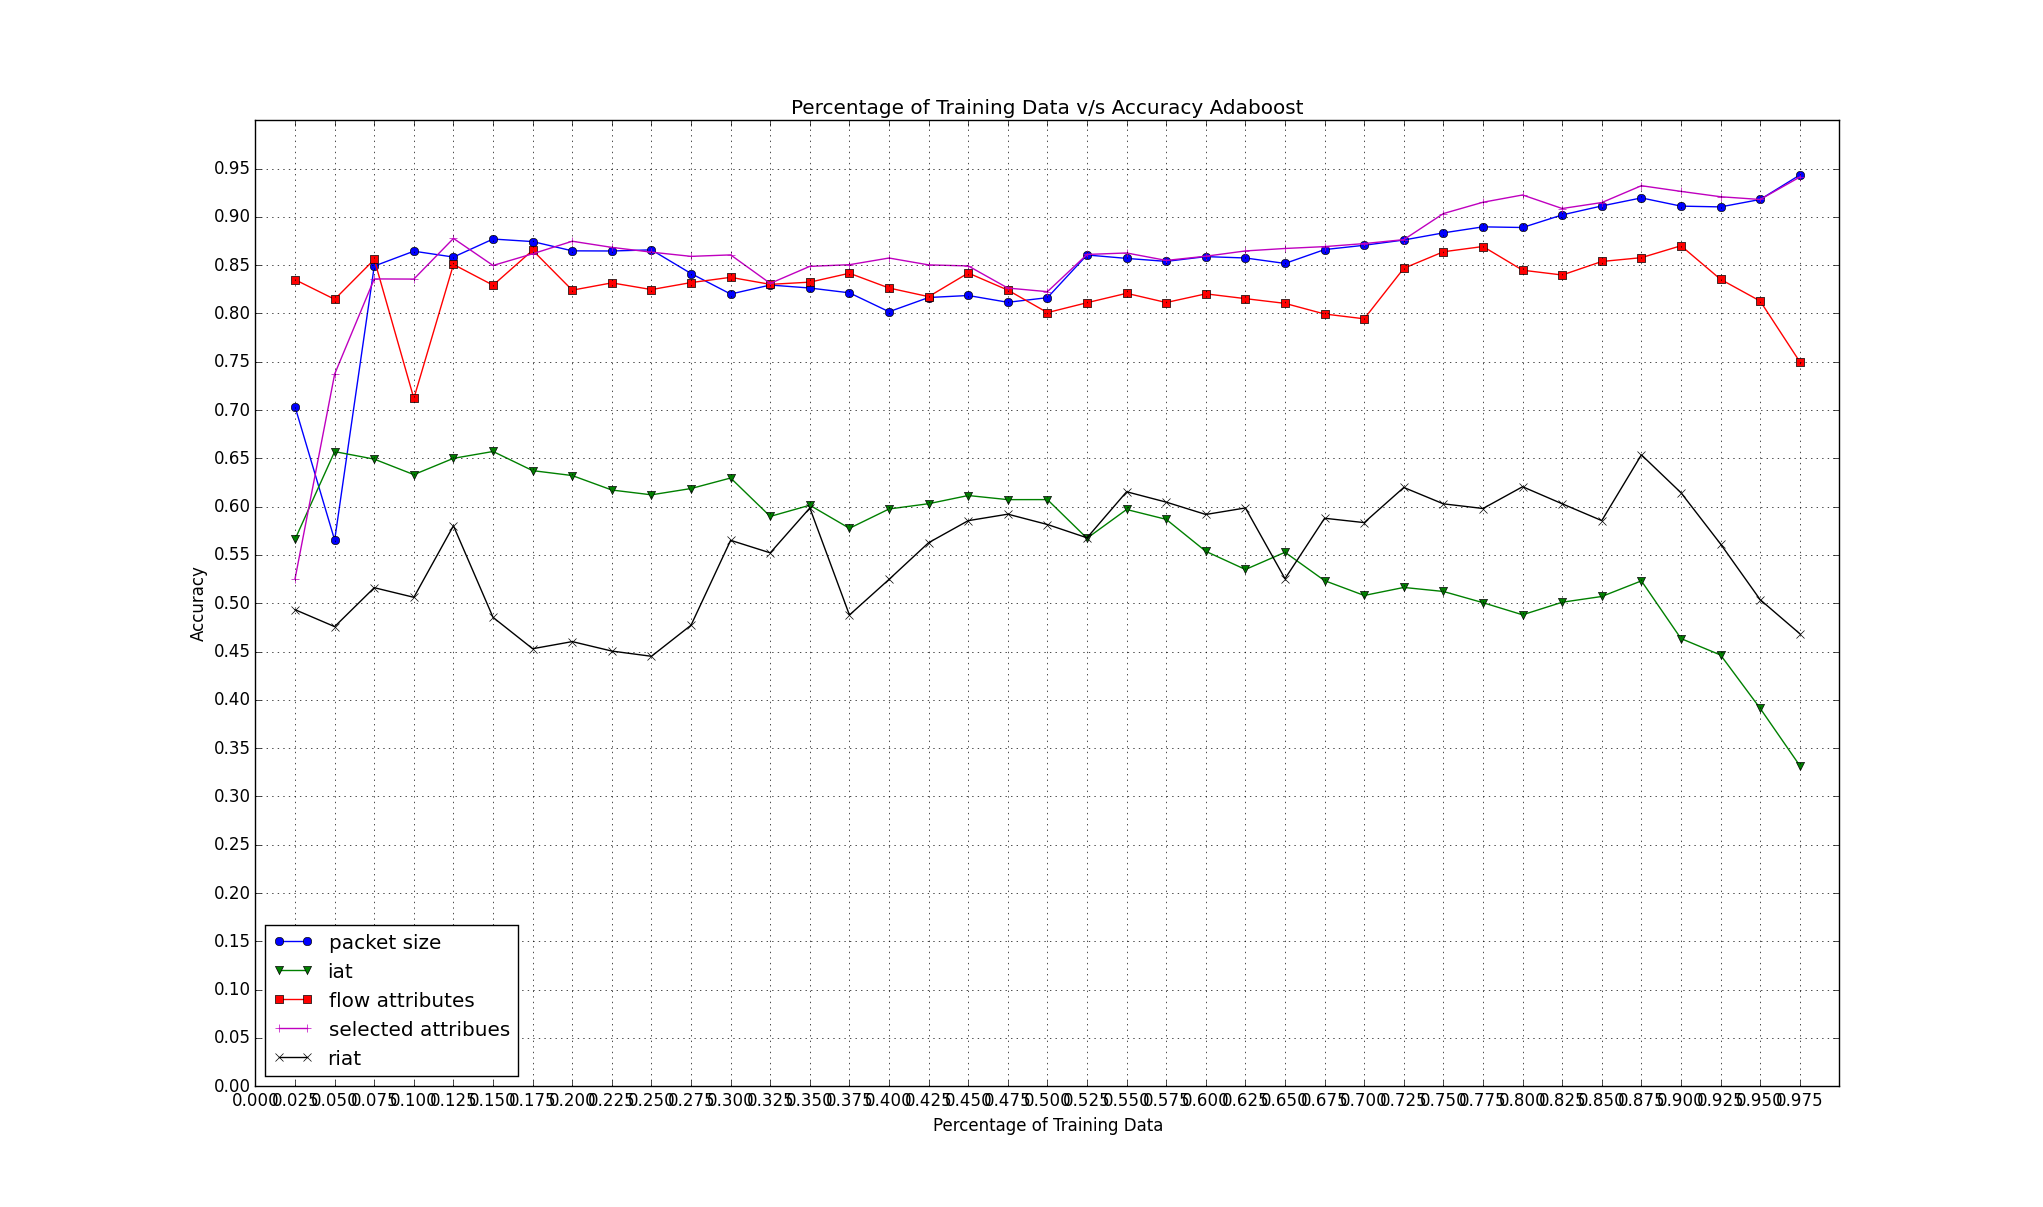
\includegraphics[width=0.45\textwidth]{adaboost_all_attr_plot.png}}
 \caption{Network traffic classification with supervised learning techniques
 }
 \label{fig:supervised}
\end{figure*}

We also conducted a set of experiments with supervised learning methods (Adaboost and Naive Bayes) with a subset of the attributes to see their impacts.
For the experiments %with the supervised learning techniques,
we considered the (i) the entire set of attributes, (ii) flow group, (iii) the packet size group, (iv) the IAT group, (v) the RIAT group, and (vi) a combination of selected attributes that showed better accuracy compared to other attributes. The selected attributes include: average packet size, minimum packet size, maximum packet size, standard deviation of packet size, total packet size, payload size, and number of packets.

%\begin{itemize}
%    \item \emph{Packet Size} This group comprised of all the packet size related attributes like \emph{average packet Size, minimum packet size, maximum packet size and standard deviation of packet size}.
%    \item \emph{IAT} This group consists of all the attributes related to IAT like \emph{average IAT, minimum IAT, maximum IAT, standard deviation of IAT}
%    \item \emph{RIAT} This group composed of all the attributes related to relative IAT like \emph{average RIAT, minimum RIAT, maximum RIAT and standard deviation of RIAT}
%    \item \emph{Flow Attributes} This group is composed of all flow level attributes like \emph{flow duration, flow size, payload size, average bytes per second, average packets per second, etc}
%    \item \emph{Selected Attributes} This group consists of selected attributes which are resulting in better accuracy than other attributes. Consists of \emph{average packet size, minimum packet size, maximum packet size, standard deviation of packet size, total packet size, payload size and number of packets}.
%\end{itemize}

Figure~\ref{fig:naive_attributes} and Figure~\ref{fig:adaboost_attributes} show the classification results with Naive Bayes and Adaboost~\cite{freund1995desicion}, respectively.
We observed Naive Bayes works poorly showing less than 60\% accuracy, and thus, we do not analyze furthermore.

Unlike this, Adaboost works well over 85\% accuracy for some combinations of attributes with 10\% or more flows in the training data set (i.e., the ratio of training and testing data sets $\ge$ 10\%).
As shown from the figure, statistics related to packet arrival time (i.e., IAT and RIAT) do not work well with the supervised classification method like using clustering.
Unlike the clustering, however, we can see that using the entire attributes works almost the best.
We also observed that using the packet size group or the selected attributes group showed outstanding performance compared to the rest of the groups, yielding comparable results with the entire attributes set group.


%From fig.\ref{fig:adaboost_attributes} we notice classification with highest accuracy at almost all the ratios of training set is observed for Adaboost. Accuracy for Naive Bayes\cite{} from fig.\ref{fig:naive_attributes} is very low when compared with Adaboost, it is not very effective in classifying the protocols.

%\begin{figure}[!t]
%	\centering
%	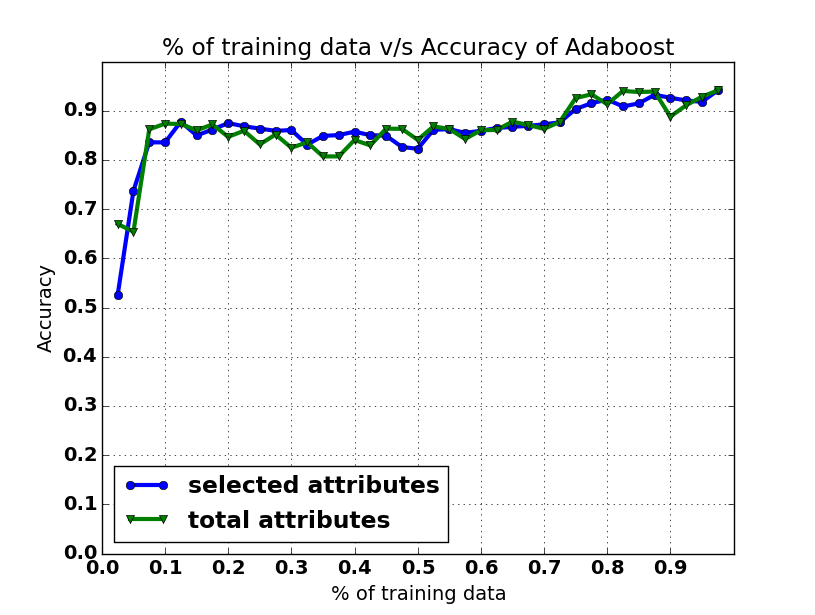
\includegraphics[width=1\columnwidth]{selected_total_attr_adaboost}
%	\caption{Percentage of Training data v/s Accuracy for Adaboost}
%	\label{adaboost_selected_total}
%\end{figure}

%Figure~\ref{adaboost_selected_total} compares Adaboost performance when using the entire data set and using the selected attributes only.
%From the figure, we observed that using the selected attributes (7 out the 18 attributes) gives us almost the same accuracy(at some points even more), as when we consider the entire 18 attributes.
%%Extra attributes is not increasing accuracy at all. With less attributes we have faster classifier. From fig.\ref{fig:k_means_all} we observe selection of subset of attributes increases accuracy dramatically.

In sum, we observed that applying the entire attributes degrades classification accuracy when using cluster-based techniques.
For supervised learning techniques, using the entire attributes does not degrade classification accuracy but using only half of the attributes showed the comparable result with the Adaboost classification technique.


\section{Multiple Cluster Models}
\label{sec:multi_cluster}

As discussed in previous sections, %Section~\ref{sec:related} and Section~\ref{sec:grouping}, 
some attributes may have greater impacts on classification accuracy for our application.
While a selected supervised learning technique works well with the entire attributes (Figure~\ref{fig:naive_attributes}), a semi-supervised learning we tested did not work well with the entire attributes showing less than 60\% accuracy (Figure~\ref{fig:k_means_all}), which is often unacceptable for network traffic classification.
However, if we apply a selected set of attributes used in Section~\ref{sec:grouping}, we observed that both supervised and semi-supervised learning techniques worked quite well, showing around 90\% accuracy.
Although not shown in Figure~\ref{fig:k_means_all}, the classification accuracy with the selected attributes we observed was around 90\%, much better than using the entire attributes.
More interesting results would be that it is possible to obtain even better accuracy up to 94\% using a clustering-based technique with only 2--4 attributes as shown from Table~\ref{table_flow_group} -- Table~\ref{table_riat_group}, which is better than the case of using the selected seven attributes altogether.

Here, a question may arise that using only a couple of attributes would always yield better results than using many more attributes and if the results would be consistent and reliable when considering a diverse range of network protocols.
For example, using only packet size statistics may work well with a certain set of network applications, but it may be degraded with a different set of applications. 
In this work, we develop a clustering-based technique that utilizes a set of attribute groups for network traffic classification.
As we observed in Table~\ref{table_flow_group} -- Table~\ref{table_riat_group}, several sets of attributes are beneficial to yield relatively high classification accuracy over 90\%.
Thus, our hypothesis is that utilizing multiple attribute groups would yield more consistent results than considering only a couple of attributes for traffic classification.
In this work, we utilize \emph{multiple} training models, each of which is from a different set of attributes, rather than simply merging the attributes together to form a \emph{single} cluster model.
In other words, multiple trained models (with different combinations of attributes) are constructed, %than one trained model (which has the superset of attributes used in training of multiple models).
and classification takes place with the constructed models, as will be described in detail next.

\begin{figure*}[!t]
	\centering
	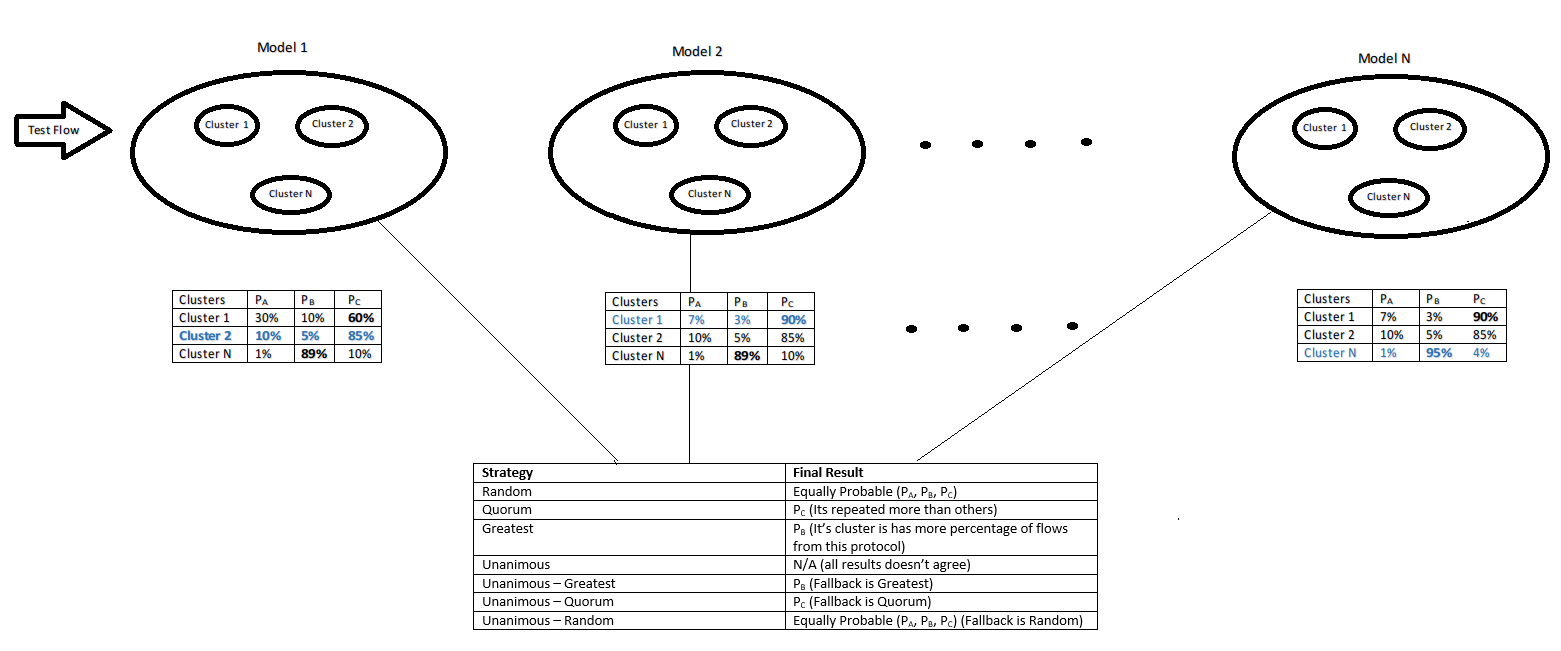
\includegraphics[width=2\columnwidth]{multi_cluster_pictorial.png}
	% where an .eps filename suffix will be assumed under latex,
	% and a .pdf suffix will be assumed for pdflatex; or what has been declared
	% via \DeclareGraphicsExtensions.
	\caption{Multi-Cluster models represented graphically.}
	\label{fig:multi_cluster_models}
\end{figure*}


With a single classifier, supervised or unsupervised, it is not possible to use multiple training models since we should put every attribute to be considered through one training model. For example, we can easily have one model based on the packet size group and the IAT group combined together, but we cannot have those two groups separately in one training model. 
%So, we advise usage of four different models, each with specific combination of attributes(one based on \emph{payload size, total packet size} other \emph{payload size, number of packets}, etc.).
If we should consider multiple training models, the key challenge is how to effectively utilize them  to reach to the final classification.
Our strategy for this question is that we use the population of each protocol in each cluster for each training model, which will be used for making the final decision.
%In this paper, we introduced a new term called population fraction, which stands for percentage of dominant application (application with most number of flows in the cluster in consideration.) flows to total flows in a cluster
In this paper, we define a new term called \emph{population fraction}, 
which stands for percentage of the flows of a protocol to the total number of flows in that cluster:

\begin{equation}
P_{prot(A)} = \Big( \frac{N_{prot(A)}}{N_{total}} \Big)
\end{equation}

Here, $P_{prot(A)}$ is the population fraction for protocol $A$, $N_{prot(A)}$ is the number of flows belonging to protocol $A$, and $N_{total}$ is the total number of flows residing in the cluster.

Figure~\ref{fig:multi_cluster_models} shows the multi-cluster models we propose in this paper. 
There can be a set of training models more than one, each of which maintains population fraction information for each protocol. % that we want to classify.
For instance, \emph{Model 1} can be constructed with attributes of average and standard deviation of packet sizes, while \emph{Model 2} can be from the number of packets and payload size attributes, and so forth.
When constructing individual models, it is straightforward to calculate population fraction  for each protocol for every cluster.



%\subsection{Description of the technique used for classification}
%Based on \ref{table_flow_group} and \ref{table_pkt_size_group} we can observe specific combination of attributes results in better accuracy(like \emph{Average Pkt Size} and \emph{Std. deviation Pkt Size}). From fig.\ref{fig:k_means_all} it can be observed that the accuracy of selected attributes is around 90\%, which can be further improved by considering multiple trained models(with different combination of attributes) than with one trained model(which has superset of combination of attributes used in training of multiple models). In a single classifier, supervised or unsupervised, we cannot consider combination of attributes as we have to put every attribute to be considered through one training model(one training model can have one combination of attributes. For example we can have one model based on \emph{packet size} group and \emph{iat} group combined together, but we cannot have \emph{iat} and \emph{packet size} group separately in one training model). So, we advise usage of four different models, each with specific combination of attributes(one based on \emph{payload size, total packet size} other \emph{payload size, number of packets}, etc.).


%After defining our four models. We have following:
%\begin{itemize}
%	\item \emph{Model 1}
%	In this model we considered attributes, Average Pkt Size and Standard Pkt Size.
%	\item \emph{Model 2}
%	We considered Average, Minimum, Maximum Packet size attributes in this model.
%	\item \emph{Model 3}
%	Considered Total Flow Size, Payload Size as the attributes for this model
%	\item \emph{Model 4}
%	Considered Number of Packets, Payload Size as the attributes for this model.
%\end{itemize}

We next describe how we can make the final classification decision from multiple models for a given input flow that needs to be classified.
From each model, it is not difficult to identify the winner that has the greatest population fraction among a set of protocols.
For example, in Figure~\ref{fig:multi_cluster_models}, Cluster 2 is selected for the test flow and we can see that $P_c$ (population fraction for protocol $C$) is the most dominant in \emph{Model} 1.
It is straightforward to make the final classification decision if all the trained models produce the identical classification result.
However, there is no guarantee for this, and it is necessary to coordinate non-identical results to reach to the final decision.

Let us define $F_{M_i}$ as the population fraction of the dominant protocol in \emph{Model i}, 
and $D_{M_i}$ as the name of the dominant protocol in the model.
Then, we get $D_{M_1} = P_c$ and $F_{M_1} = 0.8$ from Figure~\ref{fig:multi_cluster_models}, for example.

We additionally define the following two sets to represent all the outcomes from all the $N$ models:
\vspace{.2cm}

$D = \{ D_{M_i} | 1 \leq i \leq N \}$, and 

$F = \{ F_{M_i} | 1 \leq i \leq N \}$

\vspace{.2cm}

We then make use of the results from the multiple models in determining the final classification result of the incoming flow. 
To do this, we employ a set of different selection methods that chooses a model $k$ based on their own criteria function, and we accept $D_{M_k}$ as the final decision.
If the actual protocol of the test flow is $P_t$, then the classification result is:

\[ 
D_{M_k} = 
\begin{cases}
    P_t,& \text{correct classification}\\
    \text{otherwise}, & \text{incorrect classification}
\end{cases}
\]
 
We tested the following set of different strategies to select $k$:

\begin{itemize} \itemsep3pt \parskip3pt \parsep3pt
	\item \emph{Random}:
	%Select classification of any of the results from the four models as the final classification result
    Select $k$ randomly, and hence, $k = rand(N)+1$.
	\item \emph{Greatest}:
	%Select classification result from model with highest population fraction as the final classification result
    Select the greatest population fraction, that is, $k = \arg\max_i \{ F_{M_i} | 1 \leq i \leq N \}$.
	\item \emph{Quorum}:
	Select the majority result from the trained models. 
%If we have 3 models resulted in one classification result and other resulted in other application then we consider result of 3 as the final classification result. 
    In case of a tie, it falls back to \emph{Random}.
%	\item \emph{Unanimous}:
%	Select the final classification only when all the results from the trained models exactly results in the same result. Otherwise mark it as unknown
	\item \emph{Unanimous-Random}:
	Select the final classification only when all the results from the trained models are exactly the same (\emph{Unanimous}); otherwise it falls back to \emph{Random}.
	\item \emph{Unanimous-Greatest}:
	It tries \emph{Unanimous} first and falls back to \emph{Greatest} if \emph{Unanimous} has no result.
	\item \emph{Unanimous-Quorum}:
	It tries \emph{Unanimous} first and falls back to \emph{Quorum} if \emph{Unanimous} does not make a final decision.
\end{itemize}

\section{Evaluation}
\label{sec:eval}

In this section, we evaluate the proposed multi-cluster models with the selection functions to orchestrate the classification results from individual models.
We first provide a short description of the data set we used for our evaluation, then present the experimental results.
%Overall, we observed that our proposed technique works 

%\subsection{Description of the Data Set}
\subsection{Experimental Setup}

The network traffic data had been collected with full payload information in early 2014 over several months. It has been gathered on various interfaces 1) Wired, 2) WiFi, and 3) 3G and LTE. Each data set for individual applications were collected in isolation, by generating requests intentionally and capturing bidirectional data.  
To construct a flow base, we considered five tuples (i.e., source IP, destination IP, source port, destination port, and protocol), and used TCP flags to mark the start and end of a flow.
For TCP traffic, flows started before the capture or flows terminating after the capture were not considered in construction of flow information.
For UDP traffic, a fixed amount of idle time (60 seconds) was used as the indication of connection termination, as there is no connection management information for UDP flows.
A python library \emph{scapy}\cite{scapy} was used to read from \emph{pcap} files.
We then performed a refining process using  community maintained signatures~\cite{L7:2007:misc} available from L7 filters. 
We matched payload of each constructed flow with corresponding signatures from the L7 filters; any unmatched flow was discarded. % otherwise labeled as the matched signature.
We selected five protocols (http, bittorrent, http, edonkey, gnutella, and skype) that have the greatest number of flows from the flow base, as shown in Table~\ref{tab:five_protocols}.

\begin{table}
    \centering
	\caption{Protocols used for the experiments}
	\label{tab:five_protocols}
	\begin{tabular}{|c|c|c|}
		\hline Protocol & TCP/UDP & Number of flows \\ \hline
		\hline http & TCP & \\
		\hline bittorrent & TCP &  \\
		\hline edonkey & TCP &  \\
		\hline gnutella & TCP &  \\
		\hline skype & UDP &  \\
		\hline
	\end{tabular}
\end{table}

%We selected 5 protocols (Skype, Bittorrent, http, edonkey, and Gnutella) for further study, criteria for the selection of this protocols is number of flows.
%%\subsection{Cleaning}
%We constructed flows from packets, which we read from \emph{pcap} files using \emph{scapy}\cite{scapy} a python library. Used community maintained signatures\cite{L7:2007:misc} available for this protocols from L7 filters. We matched payload of each constructed flow with corresponding signatures from L7, if we find an unmatched flow then it is discarded otherwise labeled as the matched signature.


%We used \emph{sklearn}\cite{scikit-learn} a python library for machine learning algorithms in our study. \emph{sklearn}\cite{scikit-learn} is the most used python library for data analysis in python. Used \emph{Numpy}\cite{numpy} for numerical computations, it is a python library to handle numerical computation in efficient way. Used \emph{Matplotlib} for plotting the results, it is a python library which lets us plot the results.

We divide the flow data into training and testing partitions; training data to train the model and testing data to test actual classification using the trained model.
The default ratio used is 90\%:10\%, but we also explored  a variety of ratios as will be presented. 
%We used training data to train the model and testing data to test the accuracy of the trained model in correctly classifying protocols.
%During training phase we label clusters in each model(we have 4 of them) based on population fraction(majority based). Each test flow is fed into the trained model and we get the label for that test flow which is compared with the actual label for that flow. Finally
In addition, we set the default number of clusters in each trained model to 40, based on our preliminary experiments that showed less than 40 may result in unstable results.
To take variations into account, the same experiment was repeated at least five times and we report the average.
As mentioned, we used a simple metric of true positive rate for measuring classification accuracy.

%\begin{equation}
%	Accuracy = \frac{TP}{Total Flows}
%\end{equation}
% Where $TP$ stands for True positive, meaning correctly identified flow during testing. Total flows are the total number of flows in the testing set.

\subsection{Experimental Results}

We now report our observations obtained from our experiments.
We first evaluate the classification performance of the selection methods with a fixed number of trained models (4 models), and then examine the impact of the number of trained models.
We finally compare our proposed method with existing techniques.

\begin{figure}[!t]
	\centering
	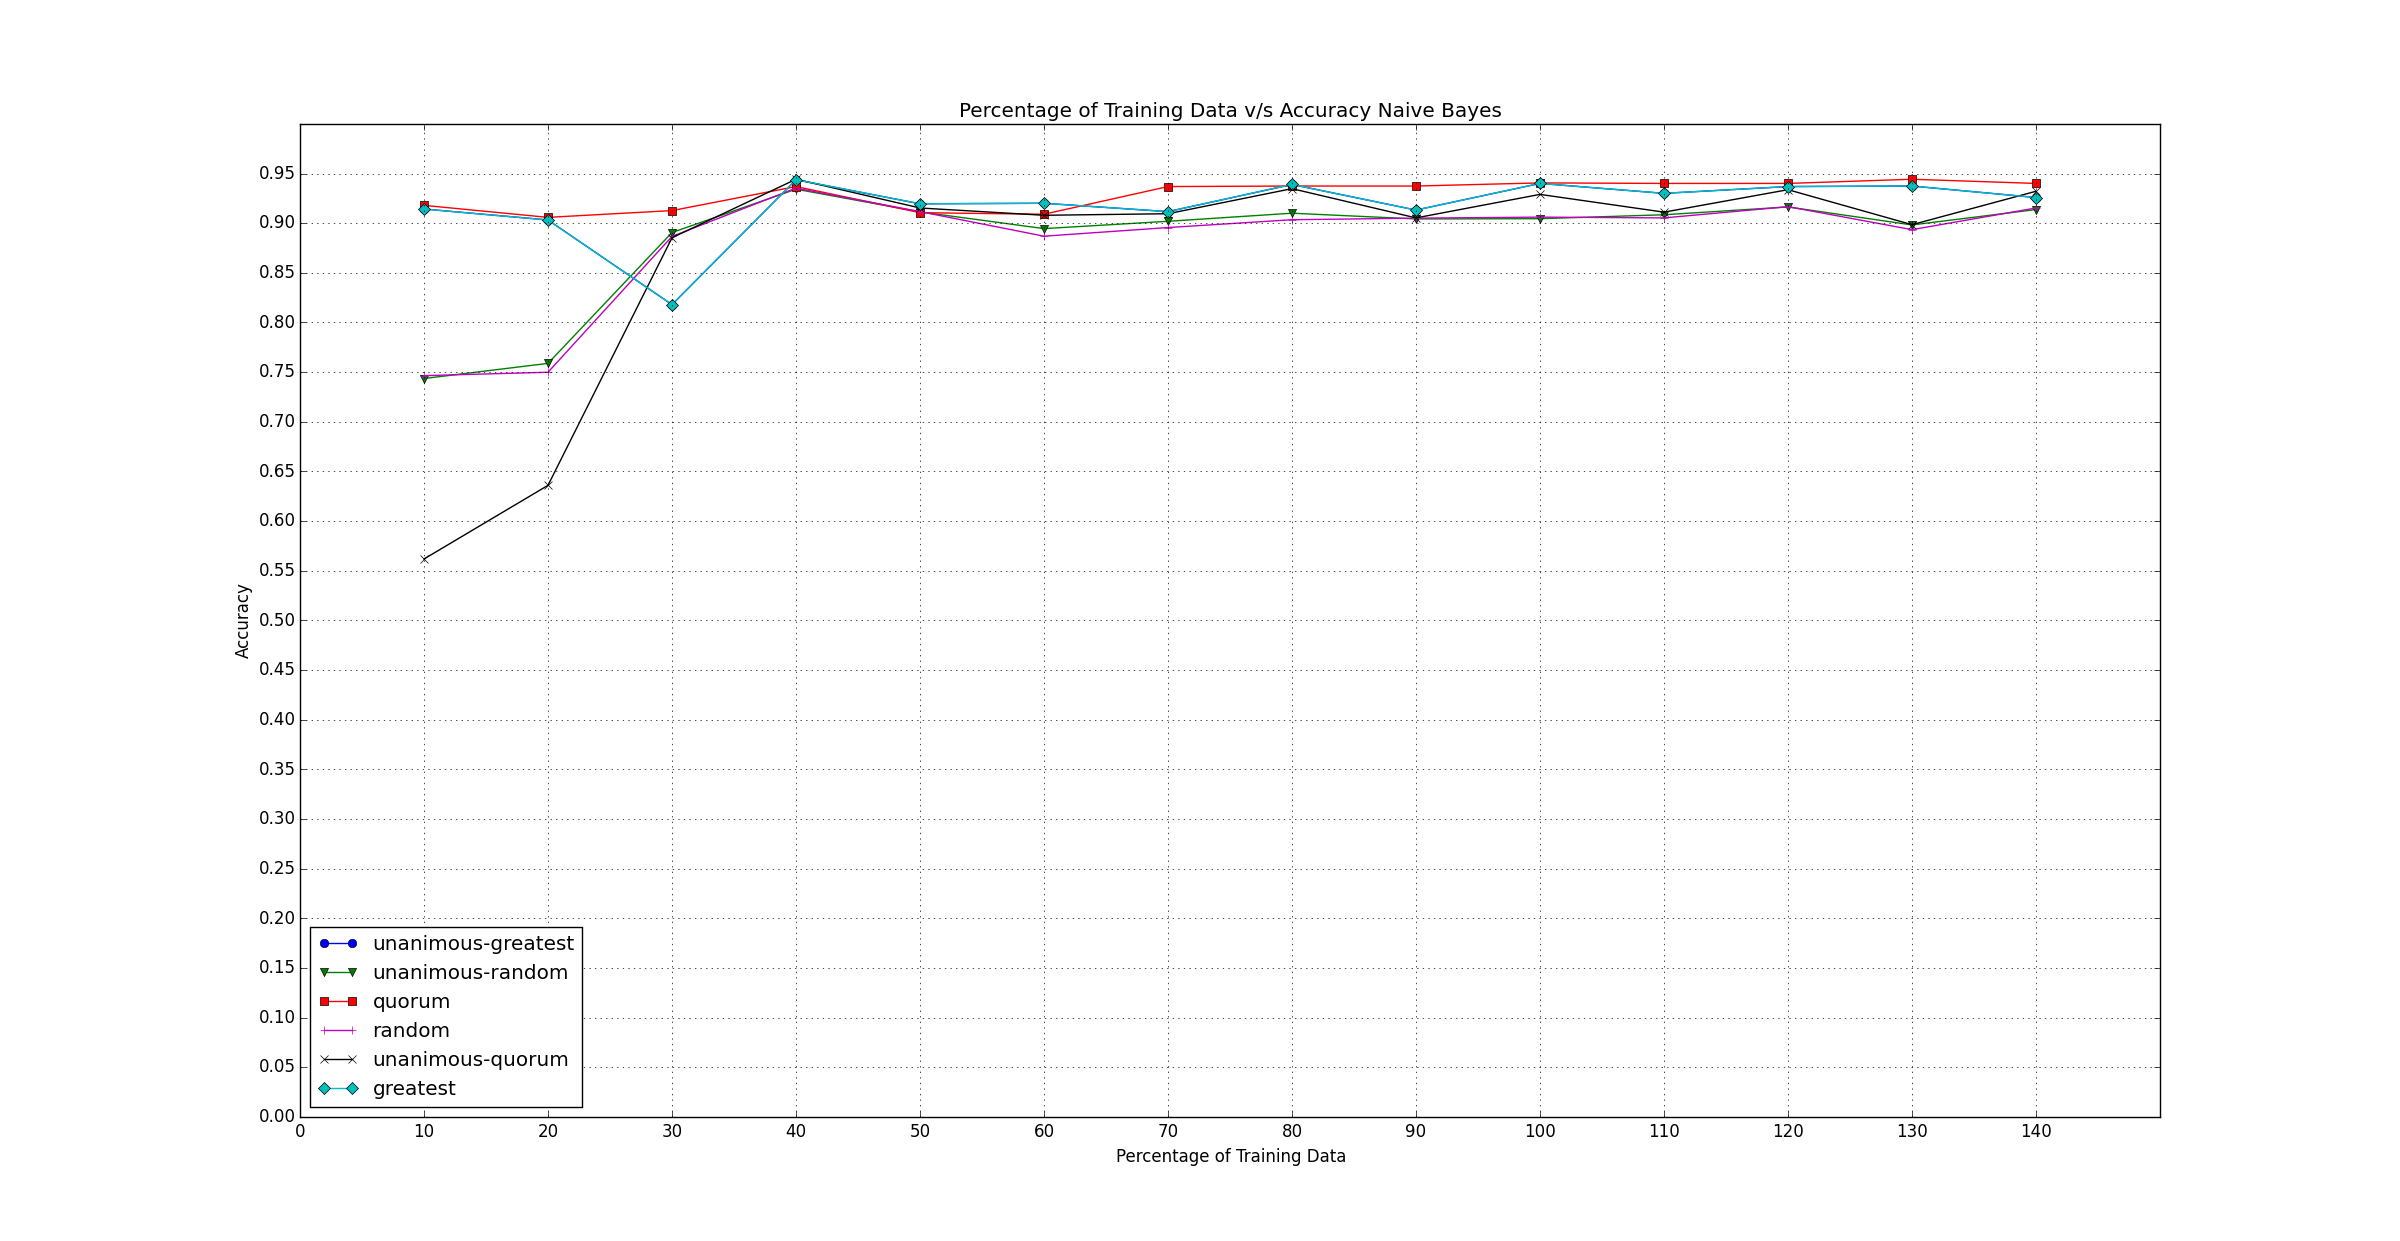
\includegraphics[width=1\columnwidth]{hypothesis_updated}
	% where an .eps filename suffix will be assumed under latex,
	% and a .pdf suffix will be assumed for pdflatex; or what has been declared
	% via \DeclareGraphicsExtensions.
	\caption{Comparison of the selection methods over different numbers of clusters}
	\label{fig:hypo_updated}
\end{figure}
%From fig.\ref{fig:hypo_updated}, it can noticed that accuracies are very high for \emph{Quorum}, \emph{Greatest} and \emph{Unanimous Greatest} strategies.

\begin{figure*}[t]
 \centering
 \subfigure[Impact of the number of clusters] {
    \label{fig:nmodels_cluster_quorum}
    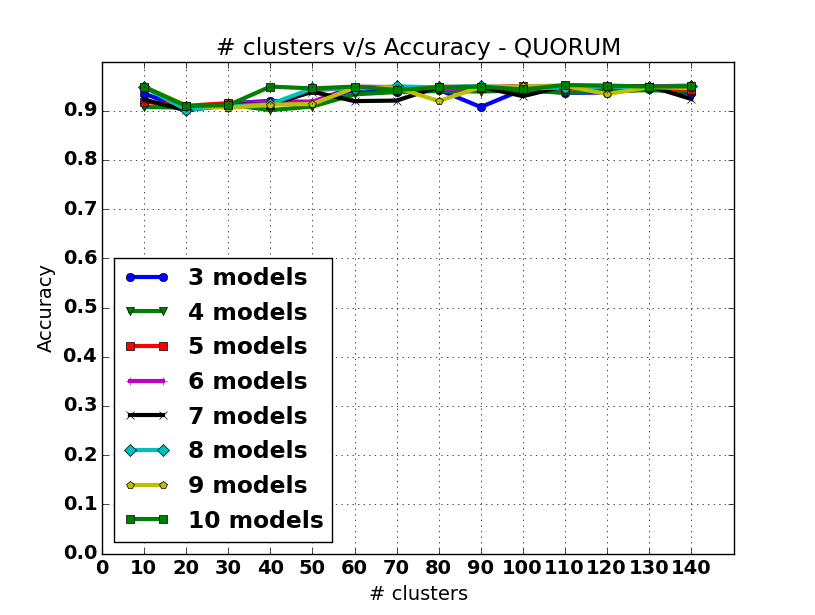
\includegraphics[width=0.45\textwidth]{nmodels_cluster_quorum}}
 \hspace{.3in}
 \subfigure[Impact of the training:testing flows ratio] {
    \label{fig:nmodels_training_quorum}
    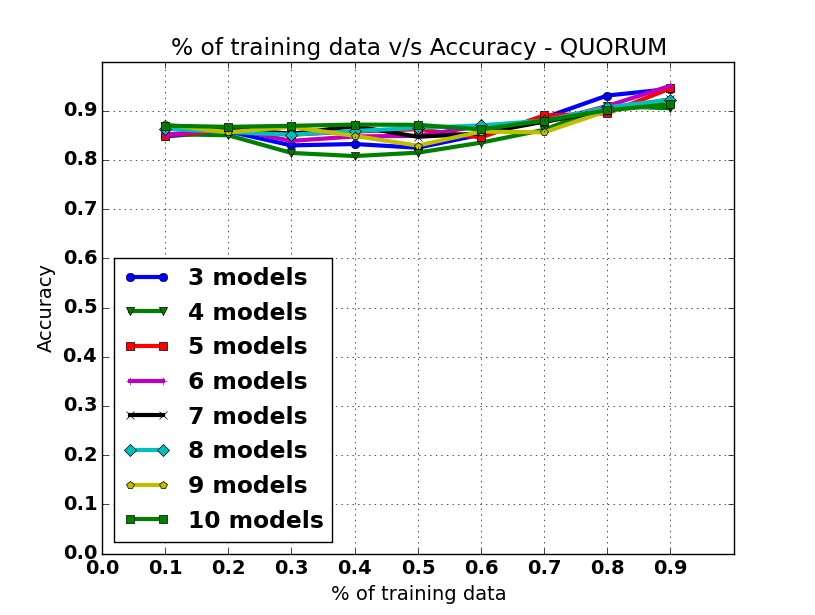
\includegraphics[width=0.45\textwidth]{nmodels_training_quorum}}
 \caption{Impact of the number of trained models
 }
 \label{fig:nmodels_quorum}
\end{figure*}


%\begin{figure*}[t]
% \centering
% \subfigure[Quorum selection] {
%    \label{fig:nmodels_cluster_quorum}
%    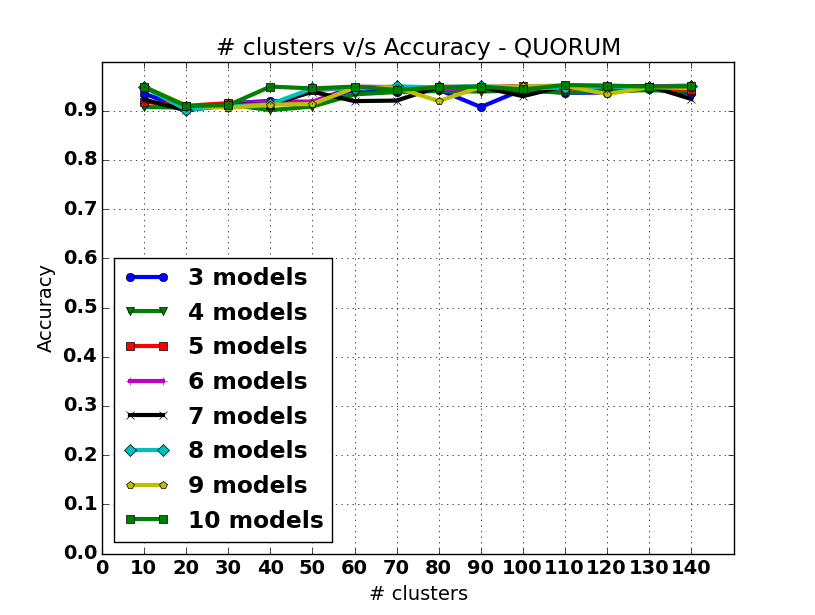
\includegraphics[width=0.45\textwidth]{nmodels_cluster_quorum}}
% \hspace{.3in}
% \subfigure[Unanimous-quorum selection] {
%    \label{fig:nmodels_cluster_unanimous_quorum}
%    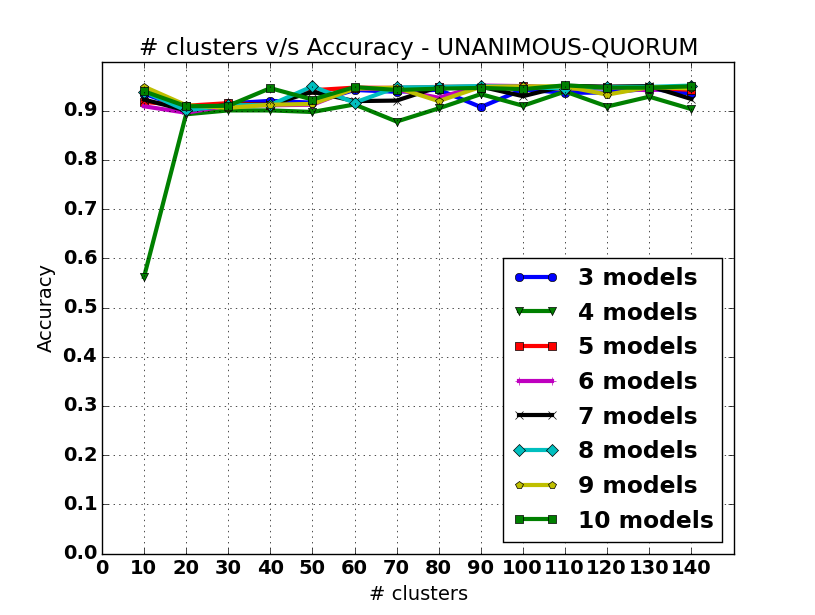
\includegraphics[width=0.45\textwidth]{nmodels_cluster_unanimous_quorum}}
% \caption{Impact of the number of clusters
% }
% \label{fig:nmodels_cluster}
%\end{figure*}
%
%\begin{figure*}[t]
% \centering
% \subfigure[Quorum selection] {
%    \label{fig:nmodels_training_quorum}
%    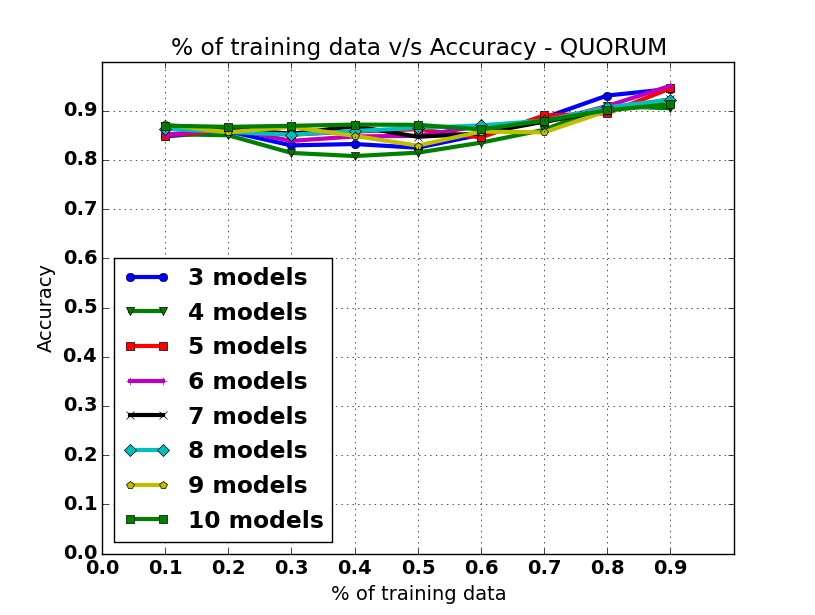
\includegraphics[width=0.45\textwidth]{nmodels_training_quorum}}
% \hspace{.3in}
% \subfigure[Unanimous-quorum selection] {
%    \label{fig:nmodels_training_unanimous_quorum}
%    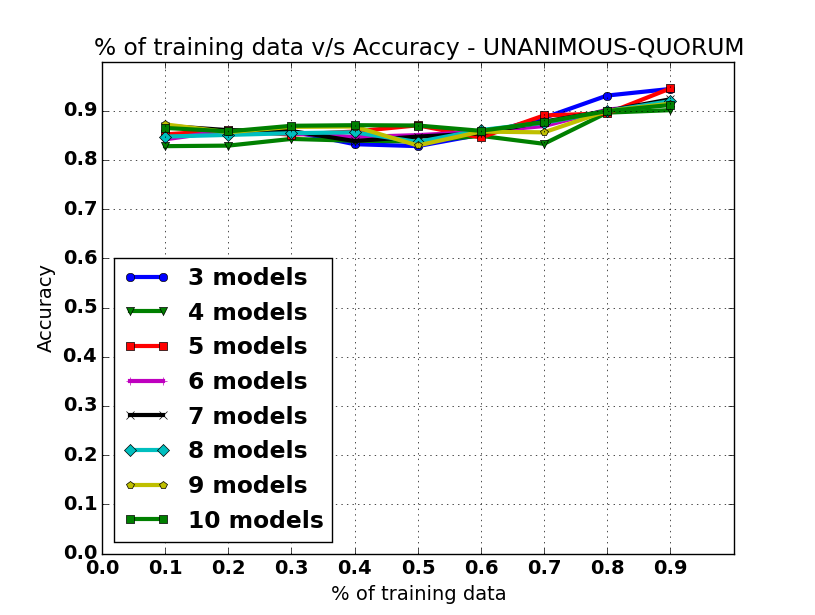
\includegraphics[width=0.45\textwidth]{nmodels_training_unanimous_quorum}}
% \caption{Impact of the size of training data set
% }
% \label{fig:nmodels_training}
%\end{figure*}


Figure~\ref{fig:hypo_updated} compares the selection methods over different numbers of clusters from 10 to 140 clusters in each training model.
For this experiment, we constructed four training models that showed the best results in Table~\ref{table_flow_group} -- Table~\ref{table_riat_group}; this is, (i) flow size and payload size, (ii) the number of packets and payload size, (iii) avg/min/max packet size, and (iv) avg/stdev packet size, for each trained model.
As can be seen from the figure, \emph{Quorum} shows quite stable results over the number of clusters, yielding over 90\% accuracy for any number of clusters.
\emph{Greatest} also shows good results but it is degraded when the number of clusters = 30, which indicates a bit more sensitive to this parameter.
\emph{Unanimous-Quorum} yields fairly stable results with 40 or greater number of clusters.
As expected, the \emph{Random} strategy is worse than the others overall.

We next explore with different numbers of trained models, varying from three to ten models.
As mentioned, the models were constructed based on the results from Table~\ref{table_flow_group} -- Table~\ref{table_riat_group}.
Since \emph{Quorum} showed fairly consistent results in Figure~\ref{fig:hypo_updated}, we selected the \emph{Quorum} strategy for this experiment.
%As shown in Figure~\ref{fig:nmodels_cluster_quorum}, there is no clear distinction with different numbers of models over the number of clusters.
%%From Figure~\ref{fig:nmodels_quorum},
%Figure~\ref{fig:nmodels_training_quorum} shows the impact of the fraction of training data flows, from 10\% to 90\% compared to the fraction of testing flows.
From Figure~\ref{fig:nmodels_quorum}, there is  no clear distinction with different numbers of trained models.
One observation is that using many more models yields slightly more stable results.
Thus, the results here indicate a potential trade-off between the training/testing complexity and classification accuracy.


%We chose \emph{Unanimous Greatest} for further study. Results for proposed classification technique, Supervised(Adaboost) and K-Means are used for comparison.
\begin{figure}[!t]
	\centering
	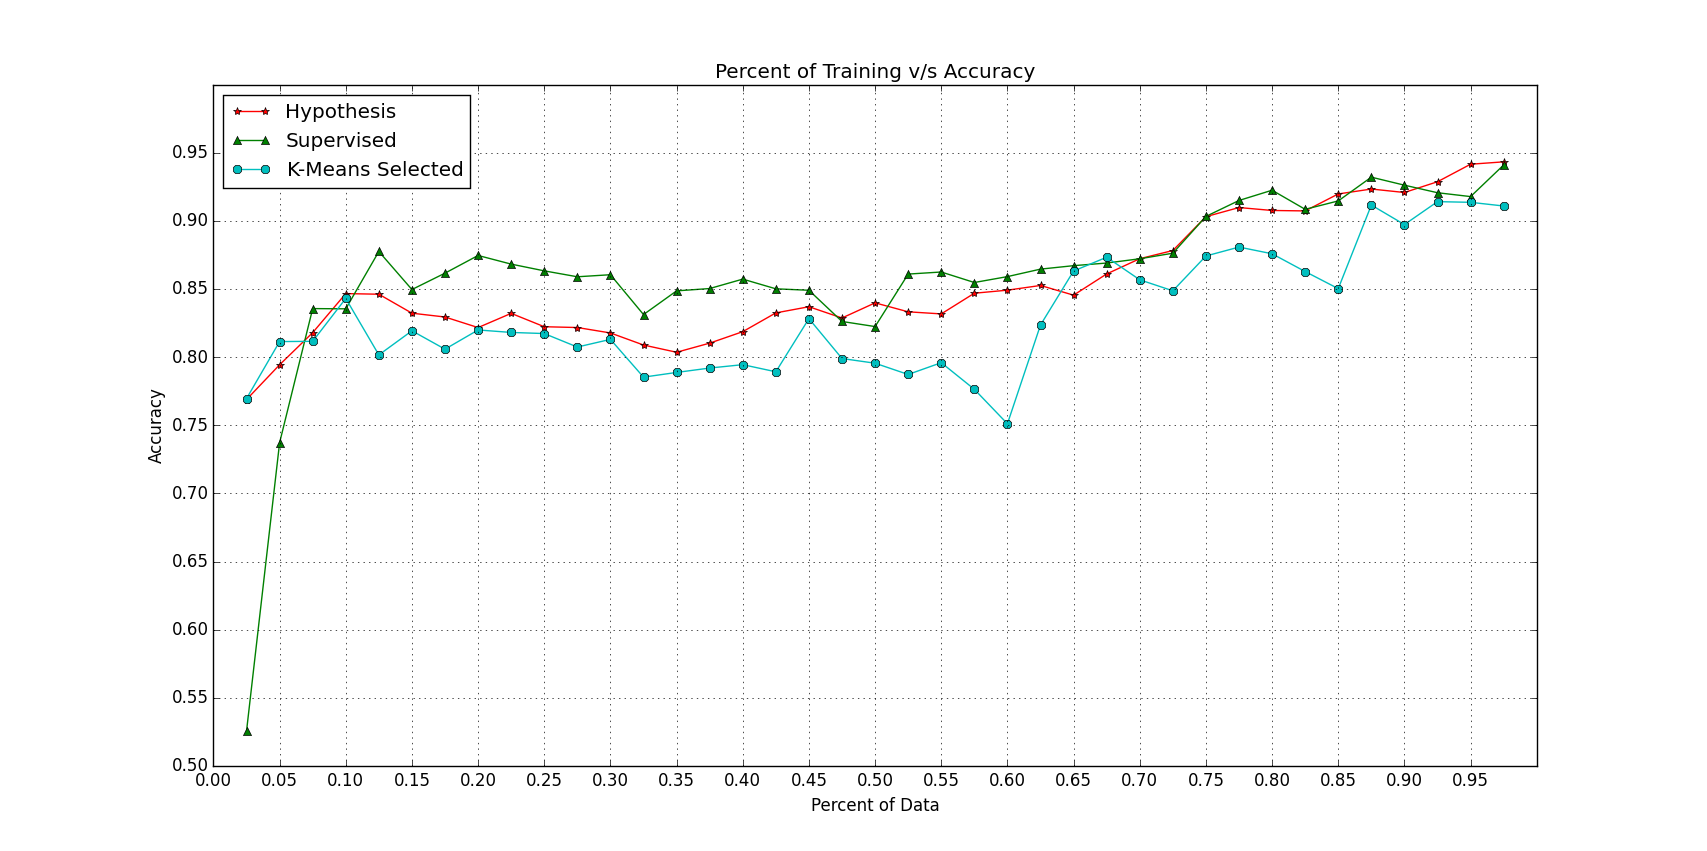
\includegraphics[width=1\columnwidth]{super_hypo_accuracy_percent_training}
	% where an .eps filename suffix will be assumed under latex,
	% and a .pdf suffix will be assumed for pdflatex; or what has been declared
	% via \DeclareGraphicsExtensions.
	\caption{Percent of training data v/s Accuracy Comparing all the existing and proposed technique}
	\label{fig:super_hypo}
\end{figure}

We finally compare our proposed technique with some of existing techniques.
In Figure~\ref{fig:super_hypo}, ``Avg Pkt Size'' is from the early identification method~\cite{Bernaille:2006:EAI:1368436.1368445}, ``K-means Selected'' from \cite{Erman:2006:TCU:1162678.1162679} with the best combination of attributes, ``Supervised'' with Adaboost with the selected attributes, and ''Proposed'' is based on our multi-cluster models with the \emph{Quorum} selection strategy.
As shown from the figure, our technique works better than ``Avg Pkt Size'' and ``K-means Selected'' that are based on clustering.
The supervised technique shows better results than the others overall, but our technique also showed almost comparable results with more than 50\% training set ratio, which indicates that the semi-supervised learning would be an comparable alternative to the supervised method.
%From fig.\ref{fig:super_hypo} we notice that the accuracy is higher than traditional K-Means clustering algorithm at almost all the ratios of the training set. Proposed technique accuracy is comparable to that of the supervised(Adaboost) technique, at times it is higher than supervised too.


% An example of a floating figure using the graphicx package.
% Note that \label must occur AFTER (or within) \caption.
% For figures, \caption should occur after the \includegraphics.
% Note that IEEEtran v1.7 and later has special internal code that
% is designed to preserve the operation of \label within \caption
% even when the captionsoff option is in effect. However, because
% of issues like this, it may be the safest practice to put all your
% \label just after \caption rather than within \caption{}.
%
% Reminder: the "draftcls" or "draftclsnofoot", not "draft", class
% option should be used if it is desired that the figures are to be
% displayed while in draft mode.
%

% Note that IEEE typically puts floats only at the top, even when this
% results in a large percentage of a column being occupied by floats.


% An example of a double column floating figure using two subfigures.
% (The subfig.sty package must be loaded for this to work.)
% The subfigure \label commands are set within each subfloat command, the
% \label for the overall figure must come after \caption.
% \hfil must be used as a separator to get equal spacing.
% The subfigure.sty package works much the same way, except \subfigure is
% used instead of \subfloat.
%
%\begin{figure*}[!t]
%\centerline{\subfloat[Case I]\includegraphics[width=2.5in]{subfigcase1}%
%\label{fig_first_case}}
%\hfil
%\subfloat[Case II]{\includegraphics[width=2.5in]{subfigcase2}%
%\label{fig_second_case}}}
%\caption{Simulation results}
%\label{fig_sim}
%\end{figure*}
%
% Note that often IEEE papers with subfigures do not employ subfigure
% captions (using the optional argument to \subfloat), but instead will
% reference/describe all of them (a), (b), etc., within the main caption.


% An example of a floating table. Note that, for IEEE style tables, the
% \caption command should come BEFORE the table. Table text will default to
% \footnotesize as IEEE normally uses this smaller font for tables.
% The \label must come after \caption as always.
%
%\begin{table}[!t]
%% increase table row spacing, adjust to taste
%\renewcommand{\arraystretch}{1.3}
% if using array.sty, it might be a good idea to tweak the value of
% \extrarowheight as needed to properly center the text within the cells
%\caption{An Example of a Table}
%\label{table_example}
%\centering
%% Some packages, such as MDW tools, offer better commands for making tables
%% than the plain LaTeX2e tabular which is used here.
%\begin{tabular}{|c||c|}
%\hline
%One & Two\\
%\hline
%Three & Four\\
%\hline
%\end{tabular}
%\end{table}


% Note that IEEE does not put floats in the very first column - or typically
% anywhere on the first page for that matter. Also, in-text middle ("here")
% positioning is not used. Most IEEE journals/conferences use top floats
% exclusively. Note that, LaTeX2e, unlike IEEE journals/conferences, places
% footnotes above bottom floats. This can be corrected via the \fnbelowfloat
% command of the stfloats package.




\section{Conclusion}
\label{sec:conc}

The importance of network traffic classification has increased for local and ISP networks for a variety of purposes including quality of service and security. Using a semi-supervised learning with clustering is one branch of research directions for traffic classification.
However, we observed fairly unacceptable results (91\% at best) with previously proposed techniques based on clustering.

In this work, we first examined the impact of attributes to the classification performance, and then 
developed a new technique that utilizes multiple trained cluster models to take multiple sets of combinations of attributes into account for classification.
The proposed technique also includes a selection step to reach to the final classification decision from the multiple models, and we explored a variety of selection strategies for this purpose.
From a set of experiments, we showed that our technique consistently outperforms the existing clustering-based methods and is fairly comparable to the supervised learning technique with Adaboost.
We also observed that the Quorum selection strategy works more consistently than the other strategies, and using many more models is slightly better with respect to stability.

This research is on the way to identify a certain set of network applications from other applications that do not need to be classified (``unknown''), which is the main reason that we chose a clustering-based model.
  


%By considering all the attributes of flow in classifying the application doesn't give better results. Selected attributes with combinations gives better accuracy. Accuracy doesn't continually increases along with number of clusters, as we get better accuracy when we are around 40 clusters.
%
%Considering IAT and RIAT for classification gives us the least accuracy when compared with other attributes of the flow. Even considering all attributes of packet size and flow also doesn't give better accuracy.
%
%Population fraction will be very good parameter in classification of flow using clustering techniques.


% conference papers do not normally have an appendix


% use section* for acknowledgement
\section*{Acknowledgment}
This work was in part supported by the IT R\&D program of MOTIE/KEIT
[10041548,
``240Gbps realtime automatic signature generation
system for application traffic classification supporting over 95\%
completeness and accuracy'']



% trigger a \newpage just before the given reference
% number - used to balance the columns on the last page
% adjust value as needed - may need to be readjusted if
% the document is modified later
%\IEEEtriggeratref{8}
% The "triggered" command can be changed if desired:
%\IEEEtriggercmd{\enlargethispage{-5in}}

% references section

% can use a bibliography generated by BibTeX as a .bbl file
% BibTeX documentation can be easily obtained at:
% http://www.ctan.org/tex-archive/biblio/bibtex/contrib/doc/
% The IEEEtran BibTeX style support page is at:
% http://www.michaelshell.org/tex/ieeetran/bibtex/
\bibliographystyle{IEEEtranS}
% argument is your BibTeX string definitions and bibliography database(s)
\bibliography{IEEEabrv,references}
%
% <OR> manually copy in the resultant .bbl file
% set second argument of \begin to the number of references
% (used to reserve space for the reference number labels box)
%\begin{thebibliography}{1}

%\bibitem{IEEEhowto:kopka}
%H.~Kopka and P.~W. Daly, \emph{A Guide to \LaTeX}, 3rd~ed.\hskip 1em plus
%  0.5em minus 0.4em\relax Harlow, England: Addison-Wesley, 1999.

%\end{thebibliography}




% that's all folks
\end{document}


